% ==============================================================================
% SECCION II: METODOLOGIA, HARDWARE Y SINTESIS DE CONTROL
% ==============================================================================
\section{Metodología, Hardware y Síntesis de Control}\label{sec:metodologia}

\subsection{Diseño Mecánico DfAM en FreeCAD 1.1}\label{subsec:dfam}
La plataforma física se diseñó paramétricamente en FreeCAD~1.1 en cuatro módulos acoplables con tornillería M3/M2, aplicando criterios de diseño para fabricación aditiva (DfAM) con cero soportes ($\text{SUP}=0$) sobre impresora Anycubic Kobra~2 (PLA de \qty{1.75}{\milli\meter}, boquilla de \qty{0.4}{\milli\meter}):
\begin{enumerate}
    \item \textbf{Base inferior y torre ($H=\qty{160}{\milli\meter}$):} Partición coaxial en $Z=\qty{70}{\milli\meter}$ (espiga $\varnothing\qty{31.6}{\milli\meter}$ a \qty{45}{\degree} y paso interno $\varnothing\qty{24}{\milli\meter}$). La base ($120\times\qty{120}{\milli\meter}$) integra cuatro aletas de refuerzo a \qty{45}{\degree}; la torre superior aloja cuatro ventanas en doble arco ojival a \qty{37.8}{\degree} para impresión invertida sobre su brida ($52\times\qty{52}{\milli\meter}$) y tapa superior desmontable.
    \item \textbf{Brazo horizontal monolítico ($L_0=\qty{88.5}{\milli\meter}$):} Viga plana con cubo en~D al eje motor y plano base en $Z=\qty{163}{\milli\meter}$ ($\qty{3.0}{\milli\meter}$ de despeje anti-roce sobre la torre), integrando canaleta superior de cables y cajera rasante para el encoder distal.
    \item \textbf{Articulación distal:} Cabezal con alojamiento en lágrima para rodamiento \texttt{608ZZ} de ajuste manual (chaflán guía \qty{45}{\degree} y ranuras de expulsión), acoplado a un eje portaimán en~D con imán diametral sin tornillos parásitos.
    \item \textbf{Barra pendular ($L_1=\qty{155}{\milli\meter}$):} Varilla coplanar con corredera de \qty{50}{\milli\meter} para el contrapeso bipartito M3 y pivote a $Z_{\text{piv}}=\qty{182.8}{\milli\meter}$, garantizando \qty{30}{\milli\meter} de despeje al plano mesa.
\end{enumerate}

Las pruebas booleanas en \texttt{freecad-py} verificaron cero interferencias en el ensamble completo ($0/23$ pares, $\qty{0.0000}{\cubic\milli\meter}$) y en el conjunto motor-encoder ($0/6$ pares). La Fig.~\ref{fig:cad_composicion} y la Tabla~\ref{tab:placas_impresion} resumen la geometría y el laminado DfAM.

\begin{figure*}[!t]
    \centering
    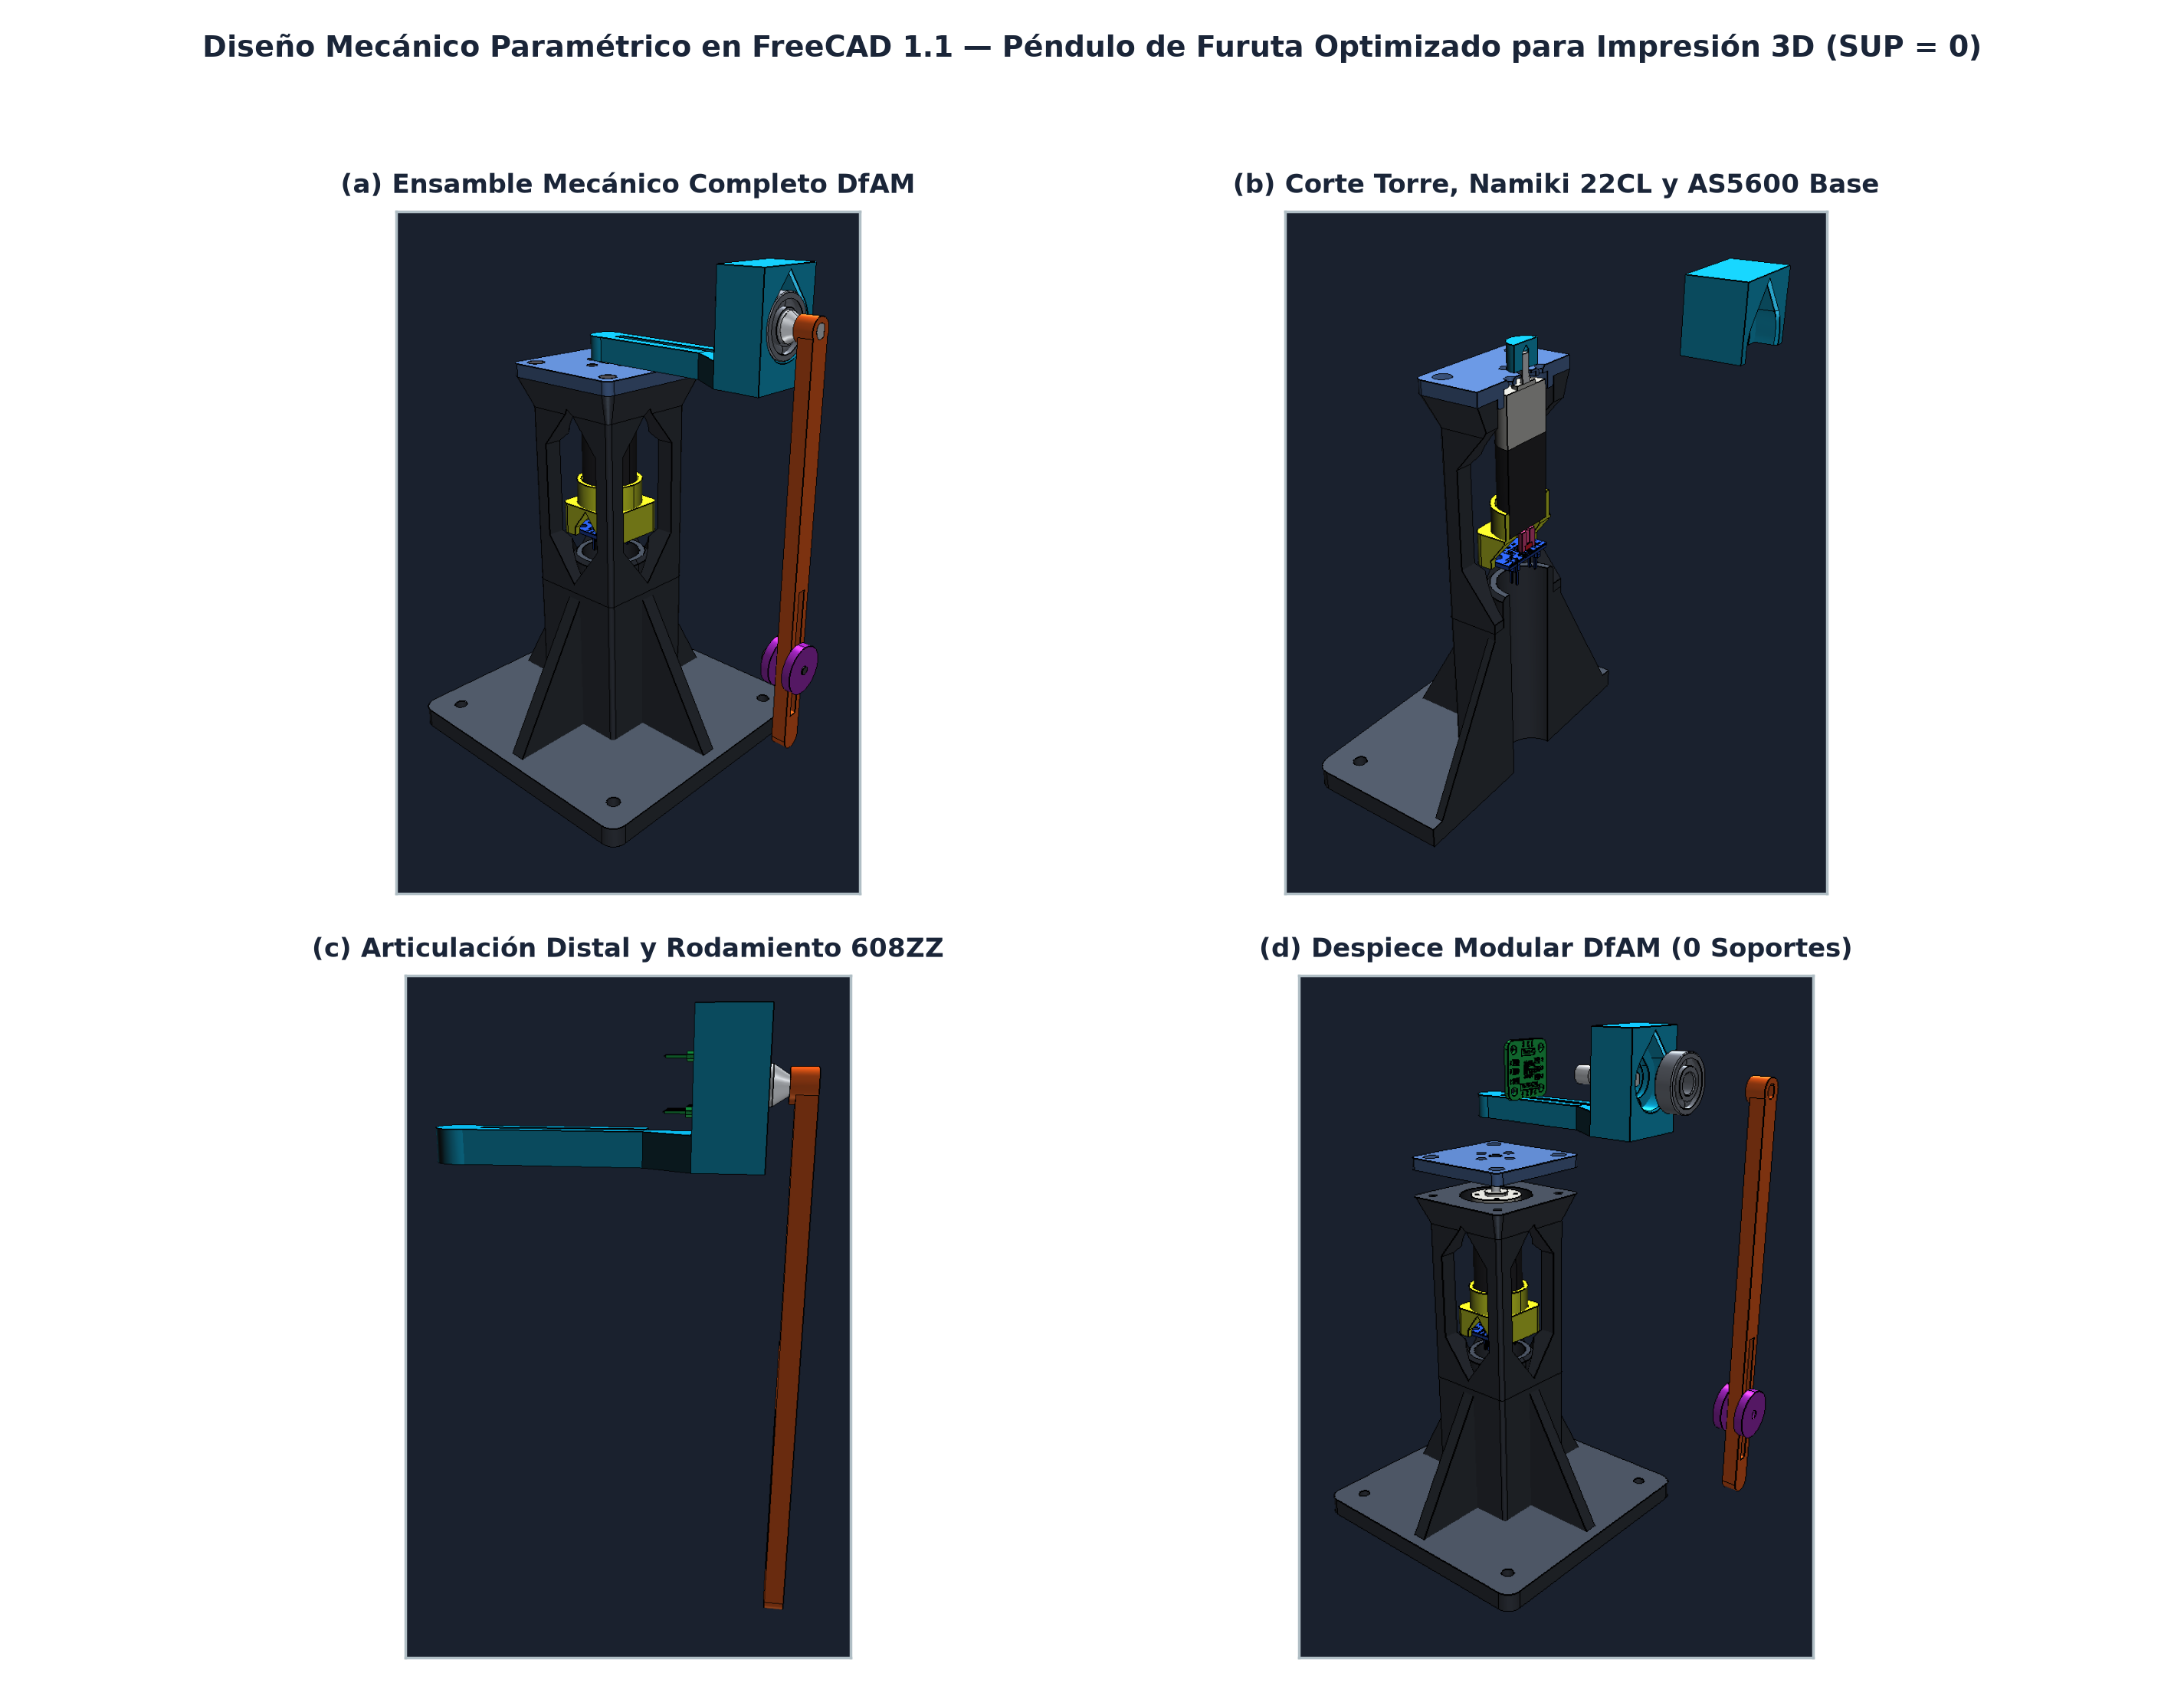
\includegraphics[width=0.92\textwidth]{fig_cad_composicion_mecanica.png}
    \caption{Composición mecánica paramétrica en FreeCAD~1.1 bajo criterios DfAM ($\text{SUP}=0$, $0/23$ colisiones): (a) ensamble completo, (b) corte de torre con motor Namiki~22CL y AS5600 base, (c) articulación distal con rodamiento \texttt{608ZZ} y (d) despiece modular.}
    \label{fig:cad_composicion}
\end{figure*}

\begin{table}[!t]
    \centering
    \caption{Placas de impresión 3D DfAM en Anycubic Kobra~2 (PLA).}
    \label{tab:placas_impresion}
    \scriptsize
    \setlength{\tabcolsep}{2.6pt}
    \begin{tabular}{@{}llccc@{}}
        \toprule
        \textbf{Placa} & \textbf{Componentes} & \textbf{Tiempo} & \textbf{Masa} & \textbf{Sop.} \\
        \midrule
        P1 & \texttt{Base\_Inferior\_Torre} & 8h 13m & \qty{107.66}{\gram} & $\text{SUP}=0$ \\
        P2 & \texttt{Torre\_Superior\_Motor} & 2h 56m & \qty{34.45}{\gram} & $\text{SUP}=0$ \\
        P3 & \texttt{Brazo\_L88, Barra, Tapa} & 2h 45m & \qty{27.42}{\gram} & $\text{SUP}=0$ \\
        P4 & \texttt{Acoplador, Eje, Portaimán} & 1h 14m & \qty{8.60}{\gram} & $\text{SUP}=0$ \\
        P5 & \texttt{Caja\_Nucleo (+Tapa)} & 3h 14m & \qty{42.16}{\gram} & $\text{SUP}=0$ \\
        P6 & \texttt{Caja\_L298N (+Tapa)} & 2h 09m & \qty{27.68}{\gram} & $\text{SUP}=0$ \\
        \midrule
        \textbf{P1--P6} & \textbf{Total sistema principal} & \textbf{20h 33m} & \textbf{\qty{247.97}{\gram}} & \textbf{0} \\
        \bottomrule
    \end{tabular}
    \vspace{2pt}
    \raggedright\scriptsize\textit{Nota:} Filamento P1--P6: \qty{83.13}{\meter}. Placa~7 opcional (ESP32): \qty{37.31}{\gram}, 2h 54m, $\text{SUP}=0$.
\end{table}

\subsection{Electrónica Embebida y Arquitectura de Pines}\label{subsec:electronica}
La unidad de control es una STM32 Nucleo-F446RE (Cortex-M4F con FPU FPv4-SP) alimentada desde \texttt{HSE\_BYPASS} (\qty{8}{\mega\hertz}) vía PLL ($M=4$, $N=180$, $P=2$) a $f_{\text{CPU}}=\qty{180}{\mega\hertz}$ con 5 estados de espera Flash \cite{STM32F446RE_Datasheet}. \texttt{TIM1\_CH1} (\texttt{PA8}, reloj \qty{180}{\mega\hertz}, $\text{PSC}=9$, $\text{ARR}=899$) genera PWM ultrasónico a \qty{20.0}{\kilo\hertz} ($0\text{--}900$ cuentas) sobre \texttt{ENA} del puente~H \texttt{L298N} (\qty{12.0}{\volt}) \cite{L298N_Datasheet}, con líneas de giro \texttt{PB4} (\texttt{IN1}), \texttt{PB5} (\texttt{IN2}) y espejos redundantes \texttt{PA9}/\texttt{PA10} en \texttt{IN2}. \texttt{TIM6} (\qty{90}{\mega\hertz}, $\text{PSC}=89$, $\text{ARR}=999$, prioridad NVIC~1) dispara la interrupción de control a \qty{1.0}{\kilo\hertz}.

Dada la dirección fija \texttt{0x36} del sensor magnético de 12~bits AS5600 \cite{ams2018}, se implementaron dos buses Soft-$\text{I}^2\text{C}$ independientes ($\sim\qty{450}{\kilo\hertz}$, lectura $< \qty{45}{\micro\second}$ con auto-detección \texttt{SCL}/\texttt{SDA} en \texttt{as5600.c}):
\begin{itemize}
    \item \textbf{Base ($\theta$, \texttt{PB8}/\texttt{PB9}):} En el rotor del motor Namiki \texttt{22CL-3501PG} previo a la reductora $80:1$, alcanzando $327\,680\text{ c/rev}$ ($\qty{0.0011}{\degree}/\text{c}$) mediante desenvolvimiento multi-vuelta.
    \item \textbf{Distal ($\alpha$, \texttt{PB10}/\texttt{PB3}):} En el pivote \texttt{608ZZ}, con resolución nativa de $4096\text{ c/rev}$ ($\qty{0.0879}{\degree}/\text{c}$).
\end{itemize}
La Fig.~\ref{fig:esquematico_electronico} detalla los 12 jumpers directos sin protoboard.

% ==============================================================================
% Figura 2: Esquemático Electrónico e Interconexión Pin a Pin
% Sistema: Péndulo Invertido Rotacional de Furuta (STM32 Nucleo-F446RE)
% Construido por restricciones geométricas relativas (positioning, calc, fit)
% ==============================================================================
\begin{figure*}[!t]
\centering
% Paleta técnica local
\definecolor{mcuBorder}{HTML}{1B3A6B}
\definecolor{mcuFill}{HTML}{F2F6FC}
\definecolor{mcuHead}{HTML}{1B3A6B}
\definecolor{pwrBorder}{HTML}{9E2A2B}
\definecolor{pwrFill}{HTML}{FDF4F4}
\definecolor{pwrHead}{HTML}{9E2A2B}
\definecolor{motBorder}{HTML}{B45309}
\definecolor{motFill}{HTML}{FFFBF0}
\definecolor{motHead}{HTML}{B45309}
\definecolor{senBorder}{HTML}{0F766E}
\definecolor{senFill}{HTML}{F0FDFA}
\definecolor{senHead}{HTML}{0F766E}
\definecolor{telBorder}{HTML}{3730A3}
\definecolor{telFill}{HTML}{F1F3FF}
\definecolor{telHead}{HTML}{3730A3}
\definecolor{wirePwr}{HTML}{B91C1C}
\definecolor{wireVcc}{HTML}{DC2626}
\definecolor{wireGnd}{HTML}{1F2937}
\definecolor{wirePwm}{HTML}{C2410C}
\definecolor{wireGpio}{HTML}{1D4ED8}
\definecolor{wireScl}{HTML}{0F766E}
\definecolor{wireSda}{HTML}{15803D}
\definecolor{wireUart}{HTML}{3730A3}
\definecolor{wireMech}{HTML}{78350F}
\definecolor{mutedTxt}{HTML}{4B5563}
\definecolor{ncColor}{HTML}{9CA3AF}
%
\resizebox{\textwidth}{!}{%
\begin{circuitikz}[
    >=Stealth,
    font=\sffamily,
    % --- Parámetros de ritmo geométrico (fuente única de verdad) ---
    /tikz/hdrnode/.style={
        rectangle,
        minimum width=#1,
        text width=\dimexpr #1 - 14pt\relax,
        align=center,
        text=white,
        inner xsep=7pt,
        inner ysep=5pt
    },
    pinlbl/.style={font=\scriptsize\ttfamily\bfseries, inner sep=1pt},
    pinsub/.style={font=\scriptsize\sffamily, text=mutedTxt, inner sep=0.5pt},
    wirelbl/.style={font=\scriptsize\sffamily\bfseries, inner sep=1.5pt},
    bushead/.style={
        font=\scriptsize\sffamily\bfseries, fill=white,
        draw=senBorder!55, rounded corners=2pt, inner xsep=5pt, inner ysep=2pt
    },
    pinport/.style={circle, fill=white, draw=black!75, line width=0.65pt, inner sep=1.35pt},
    solder/.style={circle, fill=black!85, inner sep=1.35pt},
    ncmark/.style={font=\scriptsize\bfseries, text=pwrBorder!80!black, inner sep=0pt}
]
% Dimensiones paramétricas globales
\def\mcuW{8.4cm}
\def\leftW{5.4cm}
\def\senW{5.8cm}
\def\uiW{4.0cm}
\def\stW{6.2cm}
\def\gapLeft{3.4cm}
\def\gapRight{4.0cm}
\def\rowGap{0.95cm}
\def\pinPitch{0.86cm}
\def\botGap{1.35cm}

% ==============================================================================
% 1. NODO RAÍZ: ENCABEZADO STM32 NUCLEO-F446RE
% ==============================================================================
\node[hdrnode=\mcuW, anchor=north] (mcu_hdr) at (0,0) {%
    {\small\bfseries STM32 Nucleo-F446RE}\\[1.5pt]
    {\scriptsize Cortex-M4F @ \qty{180}{\mega\hertz} \;|\; TIM6 \qty{1}{\kilo\hertz} ($T_s=\qty{1.0}{\milli\second}$)}%
};

% ==============================================================================
% 2. COLUMNA DERECHA: SENSORES AS5600 BASE (I2C1) Y DISTAL (I2C2)
% ==============================================================================
\node[hdrnode=\senW, right=\gapRight of mcu_hdr.north east, anchor=north west] (as1_hdr) {%
    {\footnotesize\bfseries Sensor 1: AS5600 Base ($\theta$)}\\[1pt]
    {\scriptsize Dir.\ \texttt{0x36} \,|\, 12 bits \,|\, Eje rotor 80:1}%
};

% Pines Sensor 1 (derivados por paso vertical relativo)
\coordinate (as1_scl) at ($(as1_hdr.south west)+(0,-0.56cm)$);
\coordinate (as1_vcc) at ($(as1_scl)+(0,-\pinPitch)$);
\coordinate (as1_sda) at ($(as1_vcc)+(0,-\pinPitch)$);
\coordinate (as1_gnd) at ($(as1_sda)+(0,-\pinPitch)$);
\coordinate (as1_bot) at ($(as1_gnd)+(0,-0.46cm)$);

\node[draw=none, fill=none, inner sep=0pt, fit=(as1_hdr)(as1_bot)] (as1) {};

% Contenido interno AS5600 Base (construcción con positioning + fit)
\node[pinlbl, anchor=west, text=wireScl] (as1_l_scl) at ($(as1_scl)+(5pt,0)$) {SCL};
\node[pinlbl, anchor=west, text=wireVcc] (as1_l_vcc) at ($(as1_vcc)+(5pt,0)$) {VCC};
\node[pinlbl, anchor=west, text=wireSda] (as1_l_sda) at ($(as1_sda)+(5pt,0)$) {SDA};
\node[pinlbl, anchor=west, text=wireGnd] (as1_l_gnd) at ($(as1_gnd)+(5pt,0)$) {GND};
\node[draw=none, fill=none, inner sep=0pt, fit=(as1_l_scl)(as1_l_vcc)(as1_l_sda)(as1_l_gnd)] (as1_lcol) {};

\node[font=\scriptsize\bfseries, text=mutedTxt, anchor=north east]
    (as1_nc_hdr) at ($(as1_hdr.south east)+(-0.14cm,-0.14cm)$) {Libres (NC)};
\coordinate (as1_nc1_y) at ($(as1_scl)!0.22!(as1_gnd)$);
\coordinate (as1_nc2_y) at ($(as1_scl)!0.58!(as1_gnd)$);
\coordinate (as1_nc3_y) at ($(as1_scl)!0.94!(as1_gnd)$);
\coordinate (as1_OUT) at (as1.east |- as1_nc1_y);
\coordinate (as1_DIR) at (as1.east |- as1_nc2_y);
\coordinate (as1_GPO) at (as1.east |- as1_nc3_y);
\node[pinlbl, anchor=east, text=mutedTxt] (as1_l_OUT) at ($(as1_OUT)+(-5pt,0)$) {OUT};
\node[pinlbl, anchor=east, text=mutedTxt] (as1_l_DIR) at ($(as1_DIR)+(-5pt,0)$) {DIR};
\node[pinlbl, anchor=east, text=mutedTxt] (as1_l_GPO) at ($(as1_GPO)+(-5pt,0)$) {GPO};
\node[draw=none, fill=none, inner sep=0pt, fit=(as1_nc_hdr)(as1_l_OUT)(as1_l_DIR)(as1_l_GPO)] (as1_rcol) {};

\coordinate (as1_div_x) at ($(as1_rcol.west)+(-0.14cm,0)$);
\coordinate (as1_div_t) at ($(as1_hdr.south)+(0,-0.10cm)$);
\coordinate (as1_div_b) at ($(as1.south)+(0,0.12cm)$);
\draw[senBorder!35, densely dotted, line width=0.65pt]
    (as1_div_x |- as1_div_t) -- (as1_div_x |- as1_div_b);

\coordinate (as1_info_r) at (as1_div_x |- as1_lcol.center);
\node[align=center, font=\scriptsize, text=senHead!85!black, text width=2.25cm]
    (as1_info) at ($(as1_lcol.east)!0.5!(as1_info_r)$)
    {Hall Magnético\\$4096\text{ c/rev}$\\\qty{3.3}{\volt} lógico};

\foreach \p in {OUT, DIR, GPO} {
    \draw[ncColor, line width=0.8pt] (as1_\p) -- ++(0.32cm,0) coordinate (as1_\p_end);
    \node[ncmark] at (as1_\p_end) {$\times$};
    \node[pinport, draw=ncColor] at (as1_\p) {};
}

% Sensor 2 (debajo de Sensor 1 con separación paramétrica \rowGap)
\node[hdrnode=\senW, below=\rowGap of as1.south west, anchor=north west] (as2_hdr) {%
    {\footnotesize\bfseries Sensor 2: AS5600 Distal ($\alpha$)}\\[1pt]
    {\scriptsize Dir.\ \texttt{0x36} \,|\, 12 bits \,|\, Eje 608ZZ}%
};

\coordinate (as2_scl) at ($(as2_hdr.south west)+(0,-0.56cm)$);
\coordinate (as2_vcc) at ($(as2_scl)+(0,-\pinPitch)$);
\coordinate (as2_sda) at ($(as2_vcc)+(0,-\pinPitch)$);
\coordinate (as2_gnd) at ($(as2_sda)+(0,-\pinPitch)$);
\coordinate (as2_bot) at ($(as2_gnd)+(0,-0.46cm)$);

\node[draw=none, fill=none, inner sep=0pt, fit=(as2_hdr)(as2_bot)] (as2) {};

\node[pinlbl, anchor=west, text=wireScl] (as2_l_scl) at ($(as2_scl)+(5pt,0)$) {SCL};
\node[pinlbl, anchor=west, text=wireVcc] (as2_l_vcc) at ($(as2_vcc)+(5pt,0)$) {VCC};
\node[pinlbl, anchor=west, text=wireSda] (as2_l_sda) at ($(as2_sda)+(5pt,0)$) {SDA};
\node[pinlbl, anchor=west, text=wireGnd] (as2_l_gnd) at ($(as2_gnd)+(5pt,0)$) {GND};
\node[draw=none, fill=none, inner sep=0pt, fit=(as2_l_scl)(as2_l_vcc)(as2_l_sda)(as2_l_gnd)] (as2_lcol) {};

\node[font=\scriptsize\bfseries, text=mutedTxt, anchor=north east]
    (as2_nc_hdr) at ($(as2_hdr.south east)+(-0.14cm,-0.14cm)$) {Libres (NC)};
\coordinate (as2_nc1_y) at ($(as2_scl)!0.22!(as2_gnd)$);
\coordinate (as2_nc2_y) at ($(as2_scl)!0.58!(as2_gnd)$);
\coordinate (as2_nc3_y) at ($(as2_scl)!0.94!(as2_gnd)$);
\coordinate (as2_OUT) at (as2.east |- as2_nc1_y);
\coordinate (as2_DIR) at (as2.east |- as2_nc2_y);
\coordinate (as2_GPO) at (as2.east |- as2_nc3_y);
\node[pinlbl, anchor=east, text=mutedTxt] (as2_l_OUT) at ($(as2_OUT)+(-5pt,0)$) {OUT};
\node[pinlbl, anchor=east, text=mutedTxt] (as2_l_DIR) at ($(as2_DIR)+(-5pt,0)$) {DIR};
\node[pinlbl, anchor=east, text=mutedTxt] (as2_l_GPO) at ($(as2_GPO)+(-5pt,0)$) {GPO};
\node[draw=none, fill=none, inner sep=0pt, fit=(as2_nc_hdr)(as2_l_OUT)(as2_l_DIR)(as2_l_GPO)] (as2_rcol) {};

\coordinate (as2_div_x) at ($(as2_rcol.west)+(-0.14cm,0)$);
\coordinate (as2_div_t) at ($(as2_hdr.south)+(0,-0.10cm)$);
\coordinate (as2_div_b) at ($(as2.south)+(0,0.12cm)$);
\draw[senBorder!35, densely dotted, line width=0.65pt]
    (as2_div_x |- as2_div_t) -- (as2_div_x |- as2_div_b);

\coordinate (as2_info_r) at (as2_div_x |- as2_lcol.center);
\node[align=center, font=\scriptsize, text=senHead!85!black, text width=2.25cm]
    (as2_info) at ($(as2_lcol.east)!0.5!(as2_info_r)$)
    {Hall Magnético\\$4096\text{ c/rev}$\\Brazo distal};

\foreach \p in {OUT, DIR, GPO} {
    \draw[ncColor, line width=0.8pt] (as2_\p) -- ++(0.32cm,0) coordinate (as2_\p_end);
    \node[ncmark] at (as2_\p_end) {$\times$};
    \node[pinport, draw=ncColor] at (as2_\p) {};
}

% ==============================================================================
% 3. COLUMNA IZQUIERDA: MOTOR DC, DRIVER PUENTE H L298N Y FUENTE 12V DC
% ==============================================================================
\node[hdrnode=\leftW, left=\gapLeft of mcu_hdr.north west, anchor=north east] (motor_hdr) {%
    {\footnotesize\bfseries Motor Namiki 22CL-3501PG}\\[1pt]
    {\scriptsize Reductor 80:1 \;|\; \qty{12}{\volt} nom.}%
};

\node[elmech, scale=0.64, fill=white, draw=motBorder, line width=0.9pt,
      below=0.38cm of motor_hdr.south] (m_sym) {M};
\coordinate (motor_bot) at ($(m_sym.south)+(0,-0.46cm)$);
\node[draw=none, fill=none, inner sep=0pt, fit=(motor_hdr)(motor_bot)] (motor) {};

% Polaridad sobre los terminales horizontales (sin tocar el cable)
\node[font=\scriptsize\bfseries, text=motHead, anchor=south east] at ($(m_sym.left)+(-3pt,2pt)$) {$+$};
\node[font=\scriptsize\bfseries, text=motHead, anchor=south west] at ($(m_sym.right)+(3pt,2pt)$) {$-$};

\coordinate (mot_out1) at ($(motor.south west)!0.26!(motor.south east)$);
\coordinate (mot_out2) at ($(motor.south west)!0.74!(motor.south east)$);
\draw[motBorder, line width=0.95pt] (m_sym.left)  -| (mot_out1);
\draw[motBorder, line width=0.95pt] (m_sym.right) -| (mot_out2);

% Driver Puente H L298N
\node[hdrnode=\leftW, below=\rowGap of motor.south west, anchor=north west] (l298_hdr) {%
    {\footnotesize\bfseries Driver Puente H L298N}\\[1pt]
    {\scriptsize Puente Darlington \;|\; TTL \qty{5}{\volt}}%
};

\coordinate (l298_ena) at ($(l298_hdr.south east)+(0,-0.50cm)$);
\coordinate (l298_in1) at ($(l298_ena)+(0,-\pinPitch)$);
\coordinate (l298_in2) at ($(l298_in1)+(0,-\pinPitch)$);
\coordinate (l298_gnd) at ($(l298_in2)+(0,-\pinPitch)$);
\coordinate (l298_bot) at ($(l298_gnd)+(0,-0.64cm)$);
\node[draw=none, fill=none, inner sep=0pt, fit=(l298_hdr)(l298_bot)] (l298n) {};

\coordinate (l298_out1) at (l298n.north -| mot_out1);
\coordinate (l298_out2) at (l298n.north -| mot_out2);
\draw[wirePwr, line width=1.25pt, ->] (l298_out1) -- (mot_out1);
\draw[wirePwr, line width=1.25pt, ->] (l298_out2) -- (mot_out2);
\node[wirelbl, text=wirePwr, anchor=east] at ($(l298_out1)!0.5!(mot_out1)+(-3pt,0)$) {OUT1};
\node[wirelbl, text=wirePwr, anchor=west] at ($(l298_out2)!0.5!(mot_out2)+( 3pt,0)$) {OUT2};

\node[pinlbl, anchor=east, text=wirePwm]  (l298_l_ena) at ($(l298_ena)+(-5pt,0)$) {ENA};
\node[pinlbl, anchor=east, text=wireGpio] (l298_l_in1) at ($(l298_in1)+(-5pt,0)$) {IN1};
\node[pinlbl, anchor=east, text=wireGpio] (l298_l_in2) at ($(l298_in2)+(-5pt,0)$) {IN2};
\node[pinlbl, anchor=east, text=wireGnd]  (l298_l_gnd) at ($(l298_gnd)+(-5pt,0)$) {GND};

\coordinate (l298_info_y) at ($(l298_ena)!0.50!(l298_in2)$);
\coordinate (l298_info_w) at (l298n.west |- l298_info_y);
\node[align=left, font=\scriptsize, text=pwrHead!85!black, text width=2.95cm, anchor=west]
    at ($(l298_info_w)+(0.22cm,0)$) {%
    \textbf{Etapa Potencia}\\
    $\bullet$ Jumper \texttt{ENA} off\\
    $\bullet$ Reg.\ \qty{5}{\volt} ON\\
    $\bullet$ $V_{\text{sat}}\!\approx\!\qty{2.0}{\volt}$
};

\coordinate (l298_vms)  at ($(l298n.south west)!0.18!(l298n.south east)$);
\coordinate (l298_pgnd) at ($(l298n.south west)!0.84!(l298n.south east)$);
\node[pinlbl, text=wirePwr, anchor=south] at ($(l298_vms)+(0,3pt)$)  {VMS};
\node[pinlbl, text=wireGnd, anchor=south] at ($(l298_pgnd)+(0,3pt)$) {GND};

% Fuente Externa 12V DC (cables en bordes sin atravesar texto; +12V interno)
\coordinate (psu_nw) at ($(l298n.south west)+(0,-\rowGap)$);
\coordinate (psu_ne) at ($(l298n.south east)+(0,-\rowGap)$);
\coordinate (psu_in_vms)  at (l298_vms |- psu_nw);
\coordinate (psu_in_gnd)  at (l298_pgnd |- psu_nw);
\coordinate (psu_src_top) at ($(psu_in_vms)+(0,-0.45cm)$);
\coordinate (psu_src_bot) at ($(psu_src_top)+(0,-1.85cm)$);
\coordinate (psu_gnd_cor) at (psu_in_gnd |- psu_src_bot);
\coordinate (psu_ne_bot)  at (psu_ne |- psu_src_bot);
\coordinate (psu_se)      at ($(psu_ne_bot)+(0,-0.45cm)$);

\node[draw=none, fill=none, inner sep=0pt, fit=(psu_nw)(psu_se)] (psu) {};

\draw[wirePwr, line width=1.25pt] (l298_vms) -- (psu_in_vms);
\node[wirelbl, text=wirePwr, anchor=west]
    at ($(l298_vms)!0.48!(psu_in_vms)+(3pt,0)$) {+\qty{12}{\volt}};

\draw[wirePwr, line width=1.10pt] (psu_in_vms) -- (psu_src_top);
\draw[wirePwr, line width=1.10pt]
    (psu_src_top) to[vsource, american, l={\scriptsize\textbf{+\qty{12}{\volt}}}] (psu_src_bot);
\draw[wireGnd, line width=1.15pt]
    (psu_src_bot) -- (psu_gnd_cor) -- (psu_in_gnd) -- (l298_pgnd);

\node[font=\footnotesize\bfseries, text=pwrHead, align=center, text width=2.25cm]
    at ($(psu_src_top)!0.50!(psu_gnd_cor)+(0.68cm,0.12cm)$) {%
    Fuente Externa\\\qty{12}{\volt} DC\\[3pt]
    {\normalfont\scriptsize\color{mutedTxt}Capacidad:\\\qty{2}{\ampere}--\qty{5}{\ampere}}%
};

% ==============================================================================
% 4. CAJA MCU CENTRAL Y TERMINALES CONECTADOS POR RESTRICCIONES ORTOGONALES
% ==============================================================================
\coordinate (mcu_bot_y)   at ($(as2.south)+(0,-0.32cm)$);
\coordinate (mcu_bot_ref) at (mcu_hdr.south |- mcu_bot_y);
\node[draw=none, fill=none, inner sep=0pt, fit=(mcu_hdr)(mcu_bot_ref)] (mcu) {};

% Proyección ortogonal de pines hacia bordes de MCU
\coordinate (mcu_scl1)  at (mcu.east |- as1_scl);
\coordinate (mcu_3v3)   at (mcu.east |- as1_vcc);
\coordinate (mcu_sda1)  at (mcu.east |- as1_sda);
\coordinate (mcu_gnd1)  at (mcu.east |- as1_gnd);

\coordinate (mcu_scl2)  at (mcu.east |- as2_scl);
\coordinate (mcu_ioref) at (mcu.east |- as2_vcc);
\coordinate (mcu_sda2)  at (mcu.east |- as2_sda);
\coordinate (mcu_gnd2)  at (mcu.east |- as2_gnd);

\coordinate (mcu_ena)   at (mcu.west |- l298_ena);
\coordinate (mcu_in1)   at (mcu.west |- l298_in1);
\coordinate (mcu_in2)   at (mcu.west |- l298_in2);
\coordinate (mcu_gnd0)  at (mcu.west |- l298_gnd);

% Etiquetas internas de pines en MCU (Derecha)
\node[pinlbl, anchor=east, text=wireScl] (mr1a) at ($(mcu_scl1)+(-5pt, 4pt)$)  {PB8 (D15)};
\node[pinsub, anchor=east]               (mr1b) at ($(mcu_scl1)+(-5pt,-4.5pt)$) {CN5-10};

\node[pinlbl, anchor=east, text=wireVcc] (mr2a) at ($(mcu_3v3)+(-5pt, 4pt)$)   {3V3};
\node[pinsub, anchor=east]               (mr2b) at ($(mcu_3v3)+(-5pt,-4.5pt)$)  {CN6-4};

\node[pinlbl, anchor=east, text=wireSda] (mr3a) at ($(mcu_sda1)+(-5pt, 4pt)$)  {PB9 (D14)};
\node[pinsub, anchor=east]               (mr3b) at ($(mcu_sda1)+(-5pt,-4.5pt)$) {CN5-9};

\node[pinlbl, anchor=east, text=wireGnd] (mr4a) at ($(mcu_gnd1)+(-5pt, 4pt)$)  {GND};
\node[pinsub, anchor=east]               (mr4b) at ($(mcu_gnd1)+(-5pt,-4.5pt)$) {CN5-7};

\node[pinlbl, anchor=east, text=wireScl] (mr5a) at ($(mcu_scl2)+(-5pt, 4pt)$)  {PB10 (D6)};
\node[pinsub, anchor=east]               (mr5b) at ($(mcu_scl2)+(-5pt,-4.5pt)$) {CN9-7};

\node[pinlbl, anchor=east, text=wireVcc] (mr6a) at ($(mcu_ioref)+(-5pt, 4pt)$) {IOREF 3.3V};
\node[pinsub, anchor=east]               (mr6b) at ($(mcu_ioref)+(-5pt,-4.5pt)$){CN6-2};

\node[pinlbl, anchor=east, text=wireSda] (mr7a) at ($(mcu_sda2)+(-5pt, 4pt)$)  {PB3 (D3)};
\node[pinsub, anchor=east]               (mr7b) at ($(mcu_sda2)+(-5pt,-4.5pt)$) {CN9-4};

\node[pinlbl, anchor=east, text=wireGnd] (mr8a) at ($(mcu_gnd2)+(-5pt, 4pt)$)  {GND};
\node[pinsub, anchor=east]               (mr8b) at ($(mcu_gnd2)+(-5pt,-4.5pt)$) {CN6-6};

% Etiquetas internas de pines en MCU (Izquierda)
\node[pinlbl, anchor=west, text=wirePwm]  (ml1a) at ($(mcu_ena)+(5pt, 4pt)$)   {PA8 (D7)};
\node[pinsub, anchor=west]                (ml1b) at ($(mcu_ena)+(5pt,-4.5pt)$)  {TIM1\_CH1 · CN9-8};

\node[pinlbl, anchor=west, text=wireGpio] (ml2a) at ($(mcu_in1)+(5pt, 4pt)$)   {PB4 (D5)};
\node[pinsub, anchor=west]                (ml2b) at ($(mcu_in1)+(5pt,-4.5pt)$)  {GPIO Out · CN9-6};

\node[pinlbl, anchor=west, text=wireGpio] (ml3a) at ($(mcu_in2)+(5pt, 4pt)$)   {PB5 (D4)};
\node[pinsub, anchor=west]                (ml3b) at ($(mcu_in2)+(5pt,-4.5pt)$)  {CN9-5 (+PA9/PA10)};

\node[pinlbl, anchor=west, text=wireGnd]  (ml4a) at ($(mcu_gnd0)+(5pt, 4pt)$)  {GND};
\node[pinsub, anchor=west]                (ml4b) at ($(mcu_gnd0)+(5pt,-4.5pt)$) {CN6-7 (común)};

% Cajas envolventes de columnas de pines para centrar mcu_core sin colisiones
\node[draw=none, fill=none, inner sep=0pt,
      fit=(ml1a)(ml1b)(ml2a)(ml2b)(ml3a)(ml3b)(ml4a)(ml4b)] (mcu_lcol) {};
\node[draw=none, fill=none, inner sep=0pt,
      fit=(mr1a)(mr1b)(mr2a)(mr2b)(mr3a)(mr3b)(mr4a)(mr4b)(mr5a)(mr5b)(mr6a)(mr6b)(mr7a)(mr7b)(mr8a)(mr8b)] (mcu_rcol) {};

\coordinate (mcu_lmid) at (mcu_lcol.east |- mcu.center);
\coordinate (mcu_rmid) at (mcu_rcol.west |- mcu.center);
\node[
    rectangle, rounded corners=3pt,
    draw=mcuBorder!45, fill=white, line width=0.75pt,
    text width=2.25cm, align=center, inner sep=4.5pt,
    font=\scriptsize
] (mcu_core) at ($(mcu_lmid)!0.5!(mcu_rmid)$) {%
    \textbf{\color{mcuHead}Periféricos}\\[3.5pt]
    \texttt{TIM1\_CH1}\\PWM \qty{20}{\kilo\hertz}\\[4pt]
    \texttt{I2C1 / I2C2}\\Soft-$\text{I}^2\text{C}$\\$\sim\qty{450}{\kilo\hertz}$\\[4pt]
    \texttt{USART2}\\DMA1\_S5\\[4pt]
    \textit{\color{mutedTxt}12 jumpers\\1-a-1 directos}
};

% ==============================================================================
% 5. BUSES DERECHOS (I2C1, I2C2) Y BUSES IZQUIERDOS (PWM/GPIO/MASA COMÚN)
% ==============================================================================
\node[bushead] at ($(mcu_scl1)!0.50!(as1_scl)+(0,0.42cm)$)
    {Bus $\text{I}^2\text{C}_1$ (Soft-$\text{I}^2\text{C}$)};
\node[bushead] at ($(mcu_scl2)!0.50!(as2_scl)+(0,0.42cm)$)
    {Bus $\text{I}^2\text{C}_2$ (Soft-$\text{I}^2\text{C}$)};

\draw[wireScl, line width=0.95pt, ->]   (mcu_scl1) -- (as1_scl);
\draw[wireVcc, line width=1.05pt]       (mcu_3v3)  -- (as1_vcc);
\draw[wireSda, line width=0.95pt, <->]  (mcu_sda1) -- (as1_sda);
\draw[wireGnd, line width=1.05pt]       (mcu_gnd1) -- (as1_gnd);

\node[wirelbl, text=wireScl, above=2pt] at ($(mcu_scl1)!0.22!(as1_scl)$) {SCL1};
\node[wirelbl, text=wireVcc, above=2pt] at ($(mcu_3v3)!0.22!(as1_vcc)$)  {\qty{3.3}{\volt}};
\node[wirelbl, text=wireSda, above=2pt] at ($(mcu_sda1)!0.22!(as1_sda)$) {SDA1};
\node[wirelbl, text=wireGnd, above=2pt] at ($(mcu_gnd1)!0.22!(as1_gnd)$) {GND};

% Pull-ups I2C1
\coordinate (pu1_scl_t) at ($(mcu_scl1)!0.54!(as1_scl)$);
\coordinate (pu1_scl_b) at ($(mcu_3v3)!0.54!(as1_vcc)$);
\coordinate (pu1_sda_t) at ($(mcu_3v3)!0.82!(as1_vcc)$);
\coordinate (pu1_sda_b) at ($(mcu_sda1)!0.82!(as1_sda)$);
\draw[senBorder!85!black, line width=0.75pt]
    (pu1_scl_t) to[R, resistors/scale=0.40] (pu1_scl_b);
\draw[senBorder!85!black, line width=0.75pt]
    (pu1_sda_t) to[R, resistors/scale=0.40] (pu1_sda_b);
\node[solder, fill=wireScl] at (pu1_scl_t) {};
\node[solder, fill=wireVcc] at (pu1_scl_b) {};
\node[solder, fill=wireVcc] at (pu1_sda_t) {};
\node[solder, fill=wireSda] at (pu1_sda_b) {};
\node[font=\scriptsize, text=senHead, anchor=west] at ($(pu1_scl_t)!0.5!(pu1_scl_b)+(4pt,0)$) {$R_{\text{pu}}$};
\node[font=\scriptsize, text=senHead, anchor=east] at ($(pu1_sda_t)!0.5!(pu1_sda_b)+(-4pt,0)$) {$R_{\text{pu}}$};
\node[font=\scriptsize\itshape, text=mutedTxt, below=6pt] at ($(mcu_gnd1)!0.68!(as1_gnd)$) {Pull-ups int./bus};

% Bus I2C2
\draw[wireScl, line width=0.95pt, ->]   (mcu_scl2)  -- (as2_scl);
\draw[wireVcc, line width=1.05pt]       (mcu_ioref) -- (as2_vcc);
\draw[wireSda, line width=0.95pt, <->]  (mcu_sda2)  -- (as2_sda);
\draw[wireGnd, line width=1.05pt]       (mcu_gnd2)  -- (as2_gnd);

\node[wirelbl, text=wireScl, above=2pt] at ($(mcu_scl2)!0.22!(as2_scl)$)  {SCL2};
\node[wirelbl, text=wireVcc, above=2pt] at ($(mcu_ioref)!0.22!(as2_vcc)$) {\qty{3.3}{\volt}};
\node[wirelbl, text=wireSda, above=2pt] at ($(mcu_sda2)!0.22!(as2_sda)$)  {SDA2};
\node[wirelbl, text=wireGnd, above=2pt] at ($(mcu_gnd2)!0.22!(as2_gnd)$)  {GND};

% Pull-ups I2C2
\coordinate (pu2_scl_t) at ($(mcu_scl2)!0.54!(as2_scl)$);
\coordinate (pu2_scl_b) at ($(mcu_ioref)!0.54!(as2_vcc)$);
\coordinate (pu2_sda_t) at ($(mcu_ioref)!0.82!(as2_vcc)$);
\coordinate (pu2_sda_b) at ($(mcu_sda2)!0.82!(as2_sda)$);
\draw[senBorder!85!black, line width=0.75pt]
    (pu2_scl_t) to[R, resistors/scale=0.40] (pu2_scl_b);
\draw[senBorder!85!black, line width=0.75pt]
    (pu2_sda_t) to[R, resistors/scale=0.40] (pu2_sda_b);
\node[solder, fill=wireScl] at (pu2_scl_t) {};
\node[solder, fill=wireVcc] at (pu2_scl_b) {};
\node[solder, fill=wireVcc] at (pu2_sda_t) {};
\node[solder, fill=wireSda] at (pu2_sda_b) {};
\node[font=\scriptsize, text=senHead, anchor=west] at ($(pu2_scl_t)!0.5!(pu2_scl_b)+(4pt,0)$) {$R_{\text{pu}}$};
\node[font=\scriptsize, text=senHead, anchor=east] at ($(pu2_sda_t)!0.5!(pu2_sda_b)+(-4pt,0)$) {$R_{\text{pu}}$};
\node[font=\scriptsize\itshape, text=mutedTxt, below=6pt] at ($(mcu_gnd2)!0.68!(as2_gnd)$) {Pull-ups int./bus};

% Buses L298N <-> MCU
\draw[wirePwm,  line width=1.15pt, ->] (mcu_ena)  -- (l298_ena);
\draw[wireGpio, line width=0.95pt, ->] (mcu_in1)  -- (l298_in1);
\draw[wireGpio, line width=0.95pt, ->] (mcu_in2)  -- (l298_in2);
\draw[wireGnd,  line width=1.15pt]     (mcu_gnd0) -- (l298_gnd);

\node[wirelbl, text=wirePwm,  above=2pt] at ($(mcu_ena)!0.50!(l298_ena)$)  {PWM \qty{20}{\kilo\hertz}};
\node[wirelbl, text=wireGpio, above=2pt] at ($(mcu_in1)!0.50!(l298_in1)$)  {IN1 (Dir.\ A)};
\node[wirelbl, text=wireGpio, above=2pt] at ($(mcu_in2)!0.50!(l298_in2)$)  {IN2 (Dir.\ B)};
\node[wirelbl, text=wireGnd,  above=2pt] at ($(l298_gnd)!0.72!(mcu_gnd0)$) {GND};

% Masa Común (estrella limpia separada de la etiqueta GND)
\coordinate (gnd_star_top) at ($(l298_gnd)!0.32!(mcu_gnd0)$);
\coordinate (gnd_psu_tap)  at ($(l298_pgnd)!0.50!(psu_in_gnd)$);
\coordinate (gnd_star_mid) at (gnd_star_top |- gnd_psu_tap);

\draw[wireGnd, line width=1.15pt] (gnd_star_top) -- (gnd_star_mid) -- (gnd_psu_tap);
\draw[wireGnd, line width=1.15pt] (gnd_star_mid) -- ++(0,-0.62cm) node[ground] (gnd_sym) {};
\node[solder, fill=wireGnd] at (gnd_star_top) {};
\node[solder, fill=wireGnd] at (gnd_psu_tap)  {};
\node[solder, fill=wireGnd] at (gnd_star_mid) {};
\node[font=\scriptsize\bfseries, text=wireGnd, align=center, below=2pt]
    at (gnd_sym.south) {Masa Común\\(GND único)};

% ==============================================================================
% 6. CORREDOR SUPERIOR: ACOPLE MECÁNICO ROTOR -> AS5600 BASE
% ==============================================================================
\coordinate (mech_start) at (motor.north);
\coordinate (mech_end)   at (as1.north);
\coordinate (mech_top_l) at ($(mech_start)+(0,0.92cm)$);
\coordinate (mech_top_r) at ($(mech_end)+(0,0.92cm)$);

\draw[wireMech, line width=1.25pt, densely dashed, ->, rounded corners=4pt]
    (mech_start) -- (mech_top_l) -- (mech_top_r) -- (mech_end);
\node[
    rectangle, rounded corners=2.5pt,
    draw=wireMech!70, fill=motFill, line width=0.8pt,
    font=\scriptsize\bfseries, text=wireMech, inner xsep=7pt, inner ysep=2.5pt
] at ($(mech_top_l)!0.50!(mech_top_r)$)
    {Acople Mecánico: Eje trasero rotor ($\varnothing\,\qty{2}{\milli\meter}$, 80:1) $\rightarrow$ Imán diametral AS5600 Base ($\theta$)};

% ==============================================================================
% 7. FILA INFERIOR: INTERFAZ NUCLEO, ST-LINK VCP Y LEYENDA
% ==============================================================================
% Bloques inferiores alineados debajo de MCU y columna derecha
\coordinate (uiblk_nw) at ($(mcu.south west)+(0,-\botGap)$);
\node[draw=none, fill=none, minimum width=\uiW, minimum height=2.25cm,
      inner sep=0pt, anchor=north west] (uiblk) at (uiblk_nw) {};

\node[hdrnode=\stW, right=0.55cm of uiblk.north east, anchor=north west] (stlink_hdr) {%
    {\footnotesize\bfseries ST-LINK VCP / PC MATLAB}%
};
\node[align=center, font=\scriptsize, text=telHead!90!black,
      text width=\dimexpr \stW - 10pt\relax,
      below=0.22cm of stlink_hdr.south] (stlink_body) {%
    UART \qty{115200}{bps} (8N1) \,|\, \texttt{USART2} + \texttt{DMA1\_S5}\\[3pt]
    Telemetría CSV (\qty{100}{\hertz}) $\leftrightarrow$ Comandos CLI/GUI%
};
\coordinate (stlink_bot_ref) at (stlink_hdr.north |- uiblk.south);
\node[draw=none, fill=none, inner sep=0pt, fit=(stlink_hdr)(stlink_body)(stlink_bot_ref)] (stlink) {};

% Interfaz Placa Nucleo: título en barra inferior para que los cables PC13/PA5 no crucen texto
\node[hdrnode=\uiW, anchor=south west] (uiblk_ftr) at (uiblk.south west) {%
    {\scriptsize\bfseries Interfaz Placa Nucleo}%
};

\coordinate (uiblk_b1_top)  at ($(uiblk.north west)!0.30!(uiblk.north east)$);
\coordinate (uiblk_ld2_top) at ($(uiblk.north west)!0.63!(uiblk.north east)$);

\coordinate (mcu_pc13) at (mcu.south -| uiblk_b1_top);
\coordinate (mcu_pa5)  at (mcu.south -| uiblk_ld2_top);

\node[pinlbl, text=telBorder, anchor=south] at ($(mcu_pc13)+(0,4pt)$) {PC13};
\node[pinlbl, text=telBorder, anchor=south] at ($(mcu_pa5)+(0,4pt)$)  {PA5};

\coordinate (b1_s1) at ($(uiblk_b1_top)+(0,-0.25cm)$);
\coordinate (b1_s2) at ($(uiblk_b1_top)+(0,-1.12cm)$);
\draw[telBorder, line width=0.95pt, <-] (mcu_pc13) -- (uiblk_b1_top);
\draw[telBorder, line width=0.85pt]    (uiblk_b1_top) -- (b1_s1)
    to[push button, switches/scale=0.52] (b1_s2) node[ground, scale=0.55] {};
\node[font=\scriptsize\bfseries, text=telHead, align=center, anchor=east]
    at ($(b1_s1)!0.48!(b1_s2)+(-7pt,0)$) {B1\\[-1pt]\normalfont\scriptsize(BTN)};

\coordinate (ld2_s1) at ($(uiblk_ld2_top)+(0,-0.25cm)$);
\coordinate (ld2_s2) at ($(uiblk_ld2_top)+(0,-1.12cm)$);
\draw[telBorder, line width=0.95pt, ->] (mcu_pa5) -- (uiblk_ld2_top);
\draw[telBorder, line width=0.85pt]    (uiblk_ld2_top) -- (ld2_s1)
    to[leD, diodes/scale=0.50, color=wireSda] (ld2_s2) node[ground, scale=0.55] {};
\node[font=\scriptsize\bfseries, text=wireSda, align=center, anchor=west]
    at ($(ld2_s1)!0.48!(ld2_s2)+(14pt,0)$) {LD2\\[-1pt]\normalfont\scriptsize(LED)};

% Pines PA2 / PA3 y cables TX / RX (DMA) con aire holgado respecto a uiblk y stlink
\coordinate (st_tx)   at ($(stlink.north west)+(0.85cm,0)$);
\coordinate (st_rx)   at ($(st_tx)+(1.80cm,0)$);
\coordinate (mcu_pa2) at (mcu.south -| st_tx);
\coordinate (mcu_pa3) at (mcu.south -| st_rx);

\node[pinlbl, text=wireUart, anchor=south] at ($(mcu_pa2)+(0,4pt)$) {PA2 (TX)};
\node[pinlbl, text=wireUart, anchor=south] at ($(mcu_pa3)+(0,4pt)$) {PA3 (RX)};

\draw[wireUart, line width=1.0pt, ->] (mcu_pa2) -- (st_tx);
\draw[wireUart, line width=1.0pt, <-] (mcu_pa3) -- (st_rx);
\node[wirelbl, text=wireUart, anchor=east] at ($(mcu_pa2)!0.50!(st_tx)+(-4pt,0)$) {TX};
\node[wirelbl, text=wireUart, anchor=west] at ($(mcu_pa3)!0.50!(st_rx)+( 4pt,0)$) {RX (DMA)};

% Leyenda de Buses y Señales (2 columnas construidas con positioning + fit: 0 solapes)
\coordinate (lg_origin) at (as2.west |- uiblk.north);
\coordinate (lg_top_e)  at (as2.east |- uiblk.north);
\node[font=\scriptsize\bfseries, text=black!85, anchor=north]
    (lg_title) at ($(lg_origin)!0.5!(lg_top_e)+(0,-0.12cm)$) {Convención de Buses y Señales};

% Columna 1 de la leyenda
\coordinate (lg_c1_r1) at ($(lg_origin)+(0.36cm,-0.62cm)$);
\draw[wirePwr, line width=1.3pt] (lg_c1_r1) -- ++(0.42cm,0) coordinate (lg_c1_e1);
\node[right=4pt, font=\scriptsize, text=black!85] (lg_t1) at (lg_c1_e1) {Potencia \qty{12}{\volt} DC};

\coordinate (lg_c1_r2) at ($(lg_c1_r1)+(0,-0.36cm)$);
\draw[wireVcc, line width=1.05pt] (lg_c1_r2) -- ++(0.42cm,0) coordinate (lg_c1_e2);
\node[right=4pt, font=\scriptsize, text=black!85] (lg_t2) at (lg_c1_e2) {Riel lógico \qty{3.3}{\volt}};

\coordinate (lg_c1_r3) at ($(lg_c1_r2)+(0,-0.36cm)$);
\draw[wireGnd, line width=1.15pt] (lg_c1_r3) -- ++(0.42cm,0) coordinate (lg_c1_e3);
\node[right=4pt, font=\scriptsize, text=black!85] (lg_t3) at (lg_c1_e3) {Masa común (GND)};

\coordinate (lg_c1_r4) at ($(lg_c1_r3)+(0,-0.36cm)$);
\draw[wireMech, line width=1.15pt, densely dashed, ->] (lg_c1_r4) -- ++(0.42cm,0) coordinate (lg_c1_e4);
\node[right=4pt, font=\scriptsize, text=black!85] (lg_t4) at (lg_c1_e4) {Acople eje};

\node[draw=none, fill=none, inner sep=0pt, fit=(lg_c1_r1)(lg_t1)(lg_t2)(lg_t3)(lg_t4)] (lg_col1) {};

% Columna 2 de la leyenda colocada dinámicamente a la derecha de lg_col1
\coordinate (lg_c2_anchor) at (lg_col1.east |- lg_c1_r1);
\coordinate (lg_c2_r1) at ($(lg_c2_anchor)+(0.46cm,0)$);
\draw[wirePwm, line width=1.15pt, ->] (lg_c2_r1) -- ++(0.42cm,0) coordinate (lg_c2_e1);
\node[right=4pt, font=\scriptsize, text=black!85] (lg_t5) at (lg_c2_e1) {PWM \qty{20}{\kilo\hertz}};

\coordinate (lg_c2_r2) at ($(lg_c2_r1)+(0,-0.36cm)$);
\draw[wireGpio, line width=0.95pt, ->] (lg_c2_r2) -- ++(0.42cm,0) coordinate (lg_c2_e2);
\node[right=4pt, font=\scriptsize, text=black!85] (lg_t6) at (lg_c2_e2) {GPIO / Control};

\coordinate (lg_c2_r3) at ($(lg_c2_r2)+(0,-0.36cm)$);
\draw[wireScl, line width=0.95pt, <->] (lg_c2_r3) -- ++(0.42cm,0) coordinate (lg_c2_e3);
\node[right=4pt, font=\scriptsize, text=black!85] (lg_t7) at (lg_c2_e3) {Soft-$\text{I}^2\text{C}$};

\coordinate (lg_c2_r4) at ($(lg_c2_r3)+(0,-0.36cm)$);
\draw[wireUart, line width=1.0pt, <->] (lg_c2_r4) -- ++(0.42cm,0) coordinate (lg_c2_e4);
\node[right=4pt, font=\scriptsize, text=black!85] (lg_t8) at (lg_c2_e4) {UART / Interfaz};

\node[draw=none, fill=none, inner sep=0pt, fit=(lg_c2_r1)(lg_t5)(lg_t6)(lg_t7)(lg_t8)] (lg_col2) {};
\coordinate (lg_se_pad) at ($(lg_col2.south east)+(0.26cm,-0.20cm)$);
\coordinate (lg_bot_ref) at (as2.east |- uiblk.south);
\node[draw=none, fill=none, inner sep=0pt, fit=(lg_origin)(lg_title)(lg_col1)(lg_col2)(lg_se_pad)(lg_bot_ref)] (legend) {};

% ==============================================================================
% 8. CAPA DE FONDO Y MARCOS (dibujados por ajuste exacto tras resolver geometría)
% ==============================================================================
\begin{scope}[on background layer]
    % MCU
    \path[fill=mcuFill, rounded corners=4pt] (mcu.north west) rectangle (mcu.south east);
    \coordinate (mcu_hb_w) at (mcu.west |- mcu_hdr.south);
    \coordinate (mcu_hb_e) at (mcu.east |- mcu_hdr.south);
    \fill[mcuHead, rounded corners=4pt] (mcu.north west) rectangle (mcu_hb_e);
    \fill[mcuHead] ($(mcu_hb_w)+(0,5pt)$) rectangle (mcu_hb_e);
    \draw[mcuBorder, rounded corners=4pt, line width=1.4pt] (mcu.north west) rectangle (mcu.south east);

    % Sensores AS5600 1 y 2
    \foreach \s in {as1, as2} {
        \path[fill=senFill, rounded corners=3.5pt] (\s.north west) rectangle (\s.south east);
        \coordinate (\s_hb_w) at (\s.west |- \s_hdr.south);
        \coordinate (\s_hb_e) at (\s.east |- \s_hdr.south);
        \fill[senHead, rounded corners=3.5pt] (\s.north west) rectangle (\s_hb_e);
        \fill[senHead] ($(\s_hb_w)+(0,5pt)$) rectangle (\s_hb_e);
        \draw[senBorder, rounded corners=3.5pt, line width=1.2pt] (\s.north west) rectangle (\s.south east);
    }

    % Motor Namiki
    \path[fill=motFill, rounded corners=3.5pt] (motor.north west) rectangle (motor.south east);
    \coordinate (mot_hb_w) at (motor.west |- motor_hdr.south);
    \coordinate (mot_hb_e) at (motor.east |- motor_hdr.south);
    \fill[motHead, rounded corners=3.5pt] (motor.north west) rectangle (mot_hb_e);
    \fill[motHead] ($(mot_hb_w)+(0,5pt)$) rectangle (mot_hb_e);
    \draw[motBorder, rounded corners=3.5pt, line width=1.2pt] (motor.north west) rectangle (motor.south east);

    % Driver L298N
    \path[fill=pwrFill, rounded corners=3.5pt] (l298n.north west) rectangle (l298n.south east);
    \coordinate (l298_hb_w) at (l298n.west |- l298_hdr.south);
    \coordinate (l298_hb_e) at (l298n.east |- l298_hdr.south);
    \fill[pwrHead, rounded corners=3.5pt] (l298n.north west) rectangle (l298_hb_e);
    \fill[pwrHead] ($(l298_hb_w)+(0,5pt)$) rectangle (l298_hb_e);
    \draw[pwrBorder, rounded corners=3.5pt, line width=1.2pt] (l298n.north west) rectangle (l298n.south east);

    % Fuente 12V DC
    \path[fill=pwrFill!65!white, rounded corners=3.5pt] (psu.north west) rectangle (psu.south east);
    \draw[pwrBorder, dashed, rounded corners=3.5pt, line width=1.0pt] (psu.north west) rectangle (psu.south east);

    % Interfaz Placa Nucleo (banda inferior oscura para aislar el texto de los cables)
    \path[fill=telFill!60!white, rounded corners=3.5pt] (uiblk.north west) rectangle (uiblk.south east);
    \coordinate (ui_ft_w) at (uiblk.west |- uiblk_ftr.north);
    \coordinate (ui_ft_e) at (uiblk.east |- uiblk_ftr.north);
    \fill[telHead!88!black, rounded corners=3.5pt] (ui_ft_w) rectangle (uiblk.south east);
    \fill[telHead!88!black] (ui_ft_w) rectangle ($(ui_ft_e)+(0,-5pt)$);
    \draw[telBorder!80!black, rounded corners=3.5pt, line width=0.95pt] (uiblk.north west) rectangle (uiblk.south east);

    % ST-LINK VCP / PC MATLAB
    \path[fill=telFill, rounded corners=3.5pt] (stlink.north west) rectangle (stlink.south east);
    \coordinate (st_hb_w) at (stlink.west |- stlink_hdr.south);
    \coordinate (st_hb_e) at (stlink.east |- stlink_hdr.south);
    \fill[telHead, rounded corners=3.5pt] (stlink.north west) rectangle (st_hb_e);
    \fill[telHead] ($(st_hb_w)+(0,5pt)$) rectangle (st_hb_e);
    \draw[telBorder, rounded corners=3.5pt, line width=1.1pt] (stlink.north west) rectangle (stlink.south east);

    % Leyenda
    \path[fill=gray!5, rounded corners=3pt] (legend.north west) rectangle (legend.south east);
    \draw[gray!65, rounded corners=3pt, line width=0.8pt] (legend.north west) rectangle (legend.south east);
\end{scope}

% Puertos de conexión circulares sobre los bordes (capa principal)
\foreach \p in {
    mcu_scl1, mcu_3v3, mcu_sda1, mcu_gnd1, as1_scl, as1_vcc, as1_sda, as1_gnd,
    mcu_scl2, mcu_ioref, mcu_sda2, mcu_gnd2, as2_scl, as2_vcc, as2_sda, as2_gnd,
    mot_out1, mot_out2, l298_out1, l298_out2, l298_vms, l298_pgnd, psu_in_vms, psu_in_gnd,
    l298_ena, l298_in1, l298_in2, l298_gnd, mcu_ena, mcu_in1, mcu_in2, mcu_gnd0,
    mcu_pc13, mcu_pa5, mcu_pa2, mcu_pa3, uiblk_b1_top, uiblk_ld2_top, st_tx, st_rx} {
    \node[pinport] at (\p) {};
}

\end{circuitikz}%
}%
\caption{Diagrama esquemático electrónico e interconexión pin a pin en la STM32 Nucleo-F446RE (12 conexiones sin protoboard): puente H L298N (\texttt{PA8} PWM \qty{20}{\kilo\hertz}, \texttt{PB4}/\texttt{PB5} con espejos \texttt{PA9}/\texttt{PA10} en \texttt{IN2}), doble bus Soft-$\text{I}^2\text{C}$ ($\sim\qty{450}{\kilo\hertz}$) para encoders AS5600 (\texttt{0x36}) y telemetría \texttt{USART2}/\texttt{DMA1\_S5}.}
\label{fig:esquematico_electronico}
\end{figure*}


\subsection{Identificación Experimental (CHAR1, CHAR2 y CHAR4)}\label{subsec:identificacion}
Desde \texttt{caracterizacion.c} se capturaron $3\,726$ muestras reales en banco (\texttt{COM13}, incluyendo validación) para identificar las no linealidades y parámetros acoplados de la planta.

\subsubsection{Zona Muerta y Compensador L298N (CHAR1)}
La rampa en lazo abierto ($918$ muestras, \qty{9.17}{\second}, Fig.~\ref{fig:exp_zona_muerta}) detectó fricción asimétrica en $+10.0\%$~CCW ($\qty{+1.20}{\volt}$) y $-21.0\%$~CW ($\qty{-2.52}{\volt}$). Para evitar ciclos límite por conmutación tipo relé, \texttt{l298n\_motor.c} aplica polaridad $\operatorname{sgn}(u)$ y magnitud lineal continua por tramos ($\text{dz}^+=9.2\%$, $\text{dz}^-=16.0\%$, rodilla $V_k=\qty{0.65}{\volt}$, $V_{\max}=\qty{12}{\volt}$):
\begin{equation}
\resizebox{0.96\columnwidth}{!}{$\displaystyle
    |\mathrm{PWM}(u)| =
    \begin{cases}
        0, & |u| < \qty{0.06}{\volt}, \\[3pt]
        \mathrm{dz}^{\pm}\dfrac{|u| - 0.06}{V_k - 0.06}, & \qty{0.06}{\volt} \le |u| < V_k, \\[6pt]
        \mathrm{dz}^{\pm} + (100 - \mathrm{dz}^{\pm})\dfrac{|u| - V_k}{V_{\max} - V_k}, & V_k \le |u| \le V_{\max}.
    \end{cases}
$}
    \label{eq:comp_l298n}
\end{equation}

\begin{figure*}[!t]
    \centering
    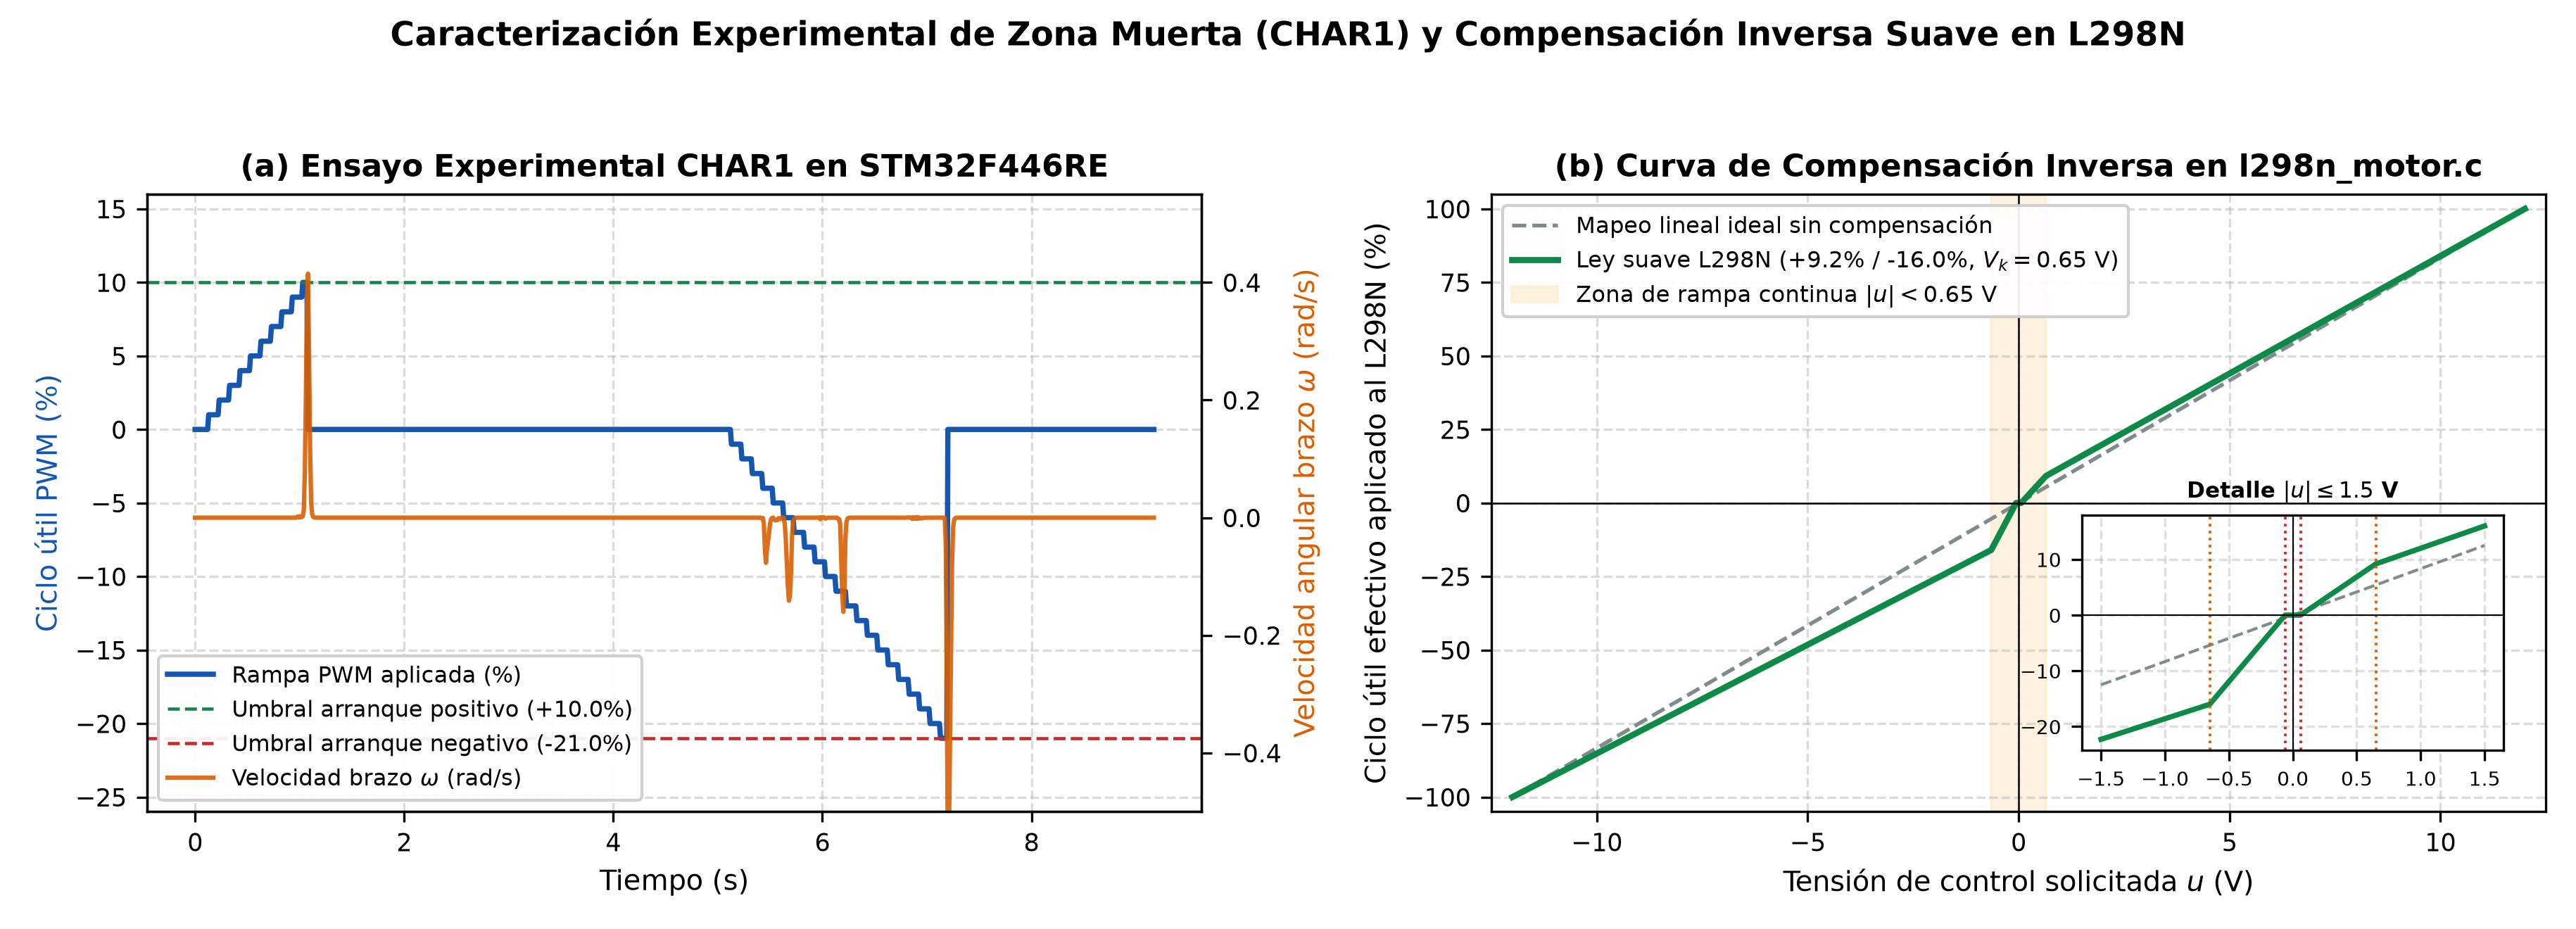
\includegraphics[width=0.86\textwidth]{fig_exp_zona_muerta_y_l298n.png}
    \caption{Ensayo CHAR1 ($918$ muestras) y curva compensadora lineal continua por tramos \eqref{eq:comp_l298n} en \texttt{l298n\_motor.c} ($+9.2\% / -16.0\%$, $V_k=\qty{0.65}{\volt}$).}
    \label{fig:exp_zona_muerta}
\end{figure*}

\subsubsection{Dinámica del Actuador Motor-Reductor (CHAR2)}
Con ocho escalones bidireccionales ($\pm 20\%\dots\pm 35\%$~PWM, $538$ muestras en \qty{5.37}{\second}, Fig.~\ref{fig:exp_motor}), el ajuste no lineal Levenberg-Marquardt obtuvo $K_v=\qty{3.3720}{(\radian\per\second)\per\volt}$ y $\tau_m=\qty{0.1175}{\second}$ ($R^2=98.51\%$, $\text{NRMSE}=87.79\%$):
\begin{equation}
    G_v(s) = \frac{\dot{\Theta}(s)}{U(s)} = \frac{3.3720}{0.1175\,s + 1}, \quad G_p(s) = \frac{3.3720}{s(0.1175\,s + 1)}.
    \label{eq:gv_identificada}
\end{equation}

\begin{figure*}[!t]
    \centering
    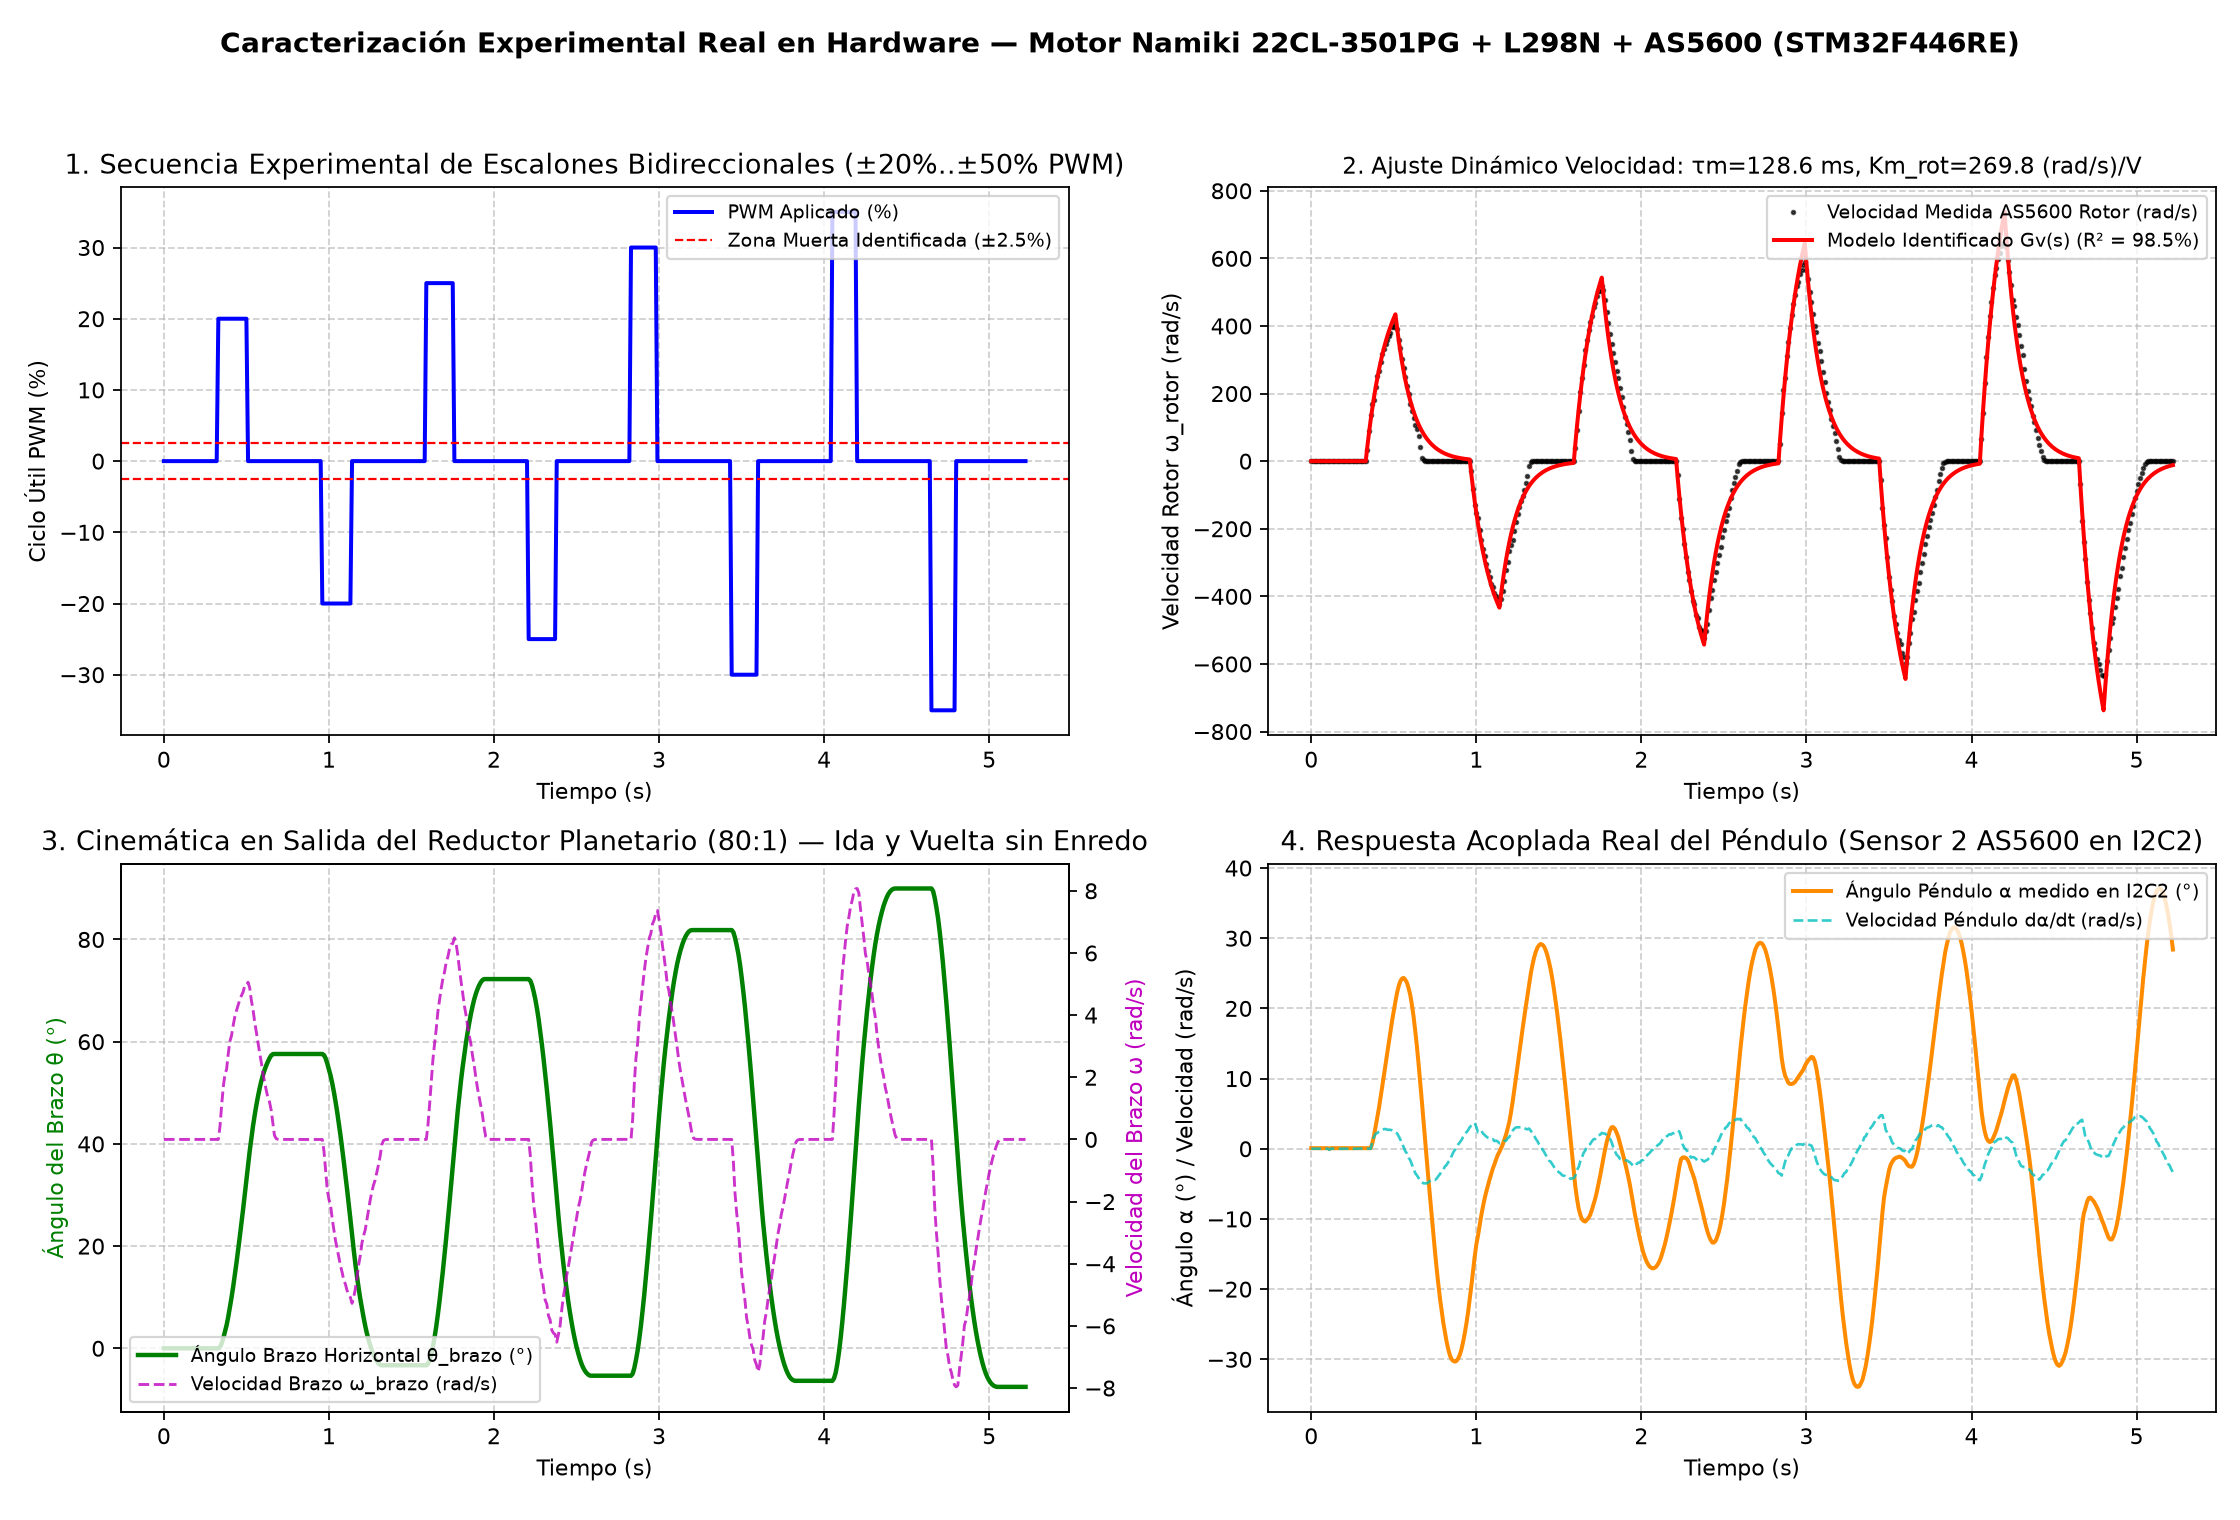
\includegraphics[width=0.74\textwidth]{fig_exp_caracterizacion_motor.png}
    \caption{Identificación CHAR2 del motor Namiki~22CL ($538$ muestras): escalones $\pm 20\%\dots\pm 35\%$~PWM, ajuste de $G_v(s)$ ($R^2=98.51\%$), salida del reductor $80:1$ y acoplamiento pendular.}
    \label{fig:exp_motor}
\end{figure*}

\subsubsection{Dinámica Acoplada y Discretización ZOH (CHAR4)}
Mediante dobletes bipolares ($+28\%/-28\%$ y $-34\%/+34\%$) seguidos de freno activo \texttt{L298N\_Brake} ($768$ muestras en \qty{7.67}{\second}, Fig.~\ref{fig:exp_sistema}), la oscilación libre ($\ddot{\theta}=0$) arrojó $\omega_n=\qty{8.8484}{\radian\per\second}$, $\zeta=0.06488$ y $K_{\text{acople}}=0.8737$. En régimen mixto viscoso-Coulomb:
\begin{equation}
    \ddot{\alpha} + 2\zeta_v\omega_n\dot{\alpha} + c_c\operatorname{sgn}(\dot{\alpha}) + \omega_n^2\sin\alpha = 0,
    \label{eq:friccion_mixta}
\end{equation}
se ajustaron $\zeta_v=0.0185$ y $c_c=\qty{0.6179}{\radian\per\second\squared}$ ($R^2=99.64\%$). Discretizando~\eqref{eq:matriz_ac}--\eqref{eq:matrices_bc_cc} por retenedor de orden cero (ZOH) a $T_s=\qty{1.0}{\milli\second}$~\cite{Franklin2015}:
\begin{equation}
\resizebox{0.96\columnwidth}{!}{$\displaystyle
    \begin{aligned}
        \mathbf{\Phi} &=
        \setlength{\arraycolsep}{3.5pt}
        \begin{bmatrix}
            1.000000 & 0.000996 & 0 & 0 \\
            0 & 0.991525 & 0 & 0 \\
            0 & 0.000004 & 1.000039 & 0.000999 \\
            0 & 0.007400 & 0.078250 & 0.998892
        \end{bmatrix}, \\
        \mathbf{\Gamma} &= \begin{bmatrix} 0.000014 & 0.028576 & -0.000012 & -0.024953 \end{bmatrix}^T,
    \end{aligned}
$}
    \label{eq:zoh_discreto}
\end{equation}
con valores propios $\lambda(\mathbf{\Phi})=\{1.000000,\, 0.991525,\, 0.990603,\, 1.008327\}$.

\begin{figure*}[!t]
    \centering
    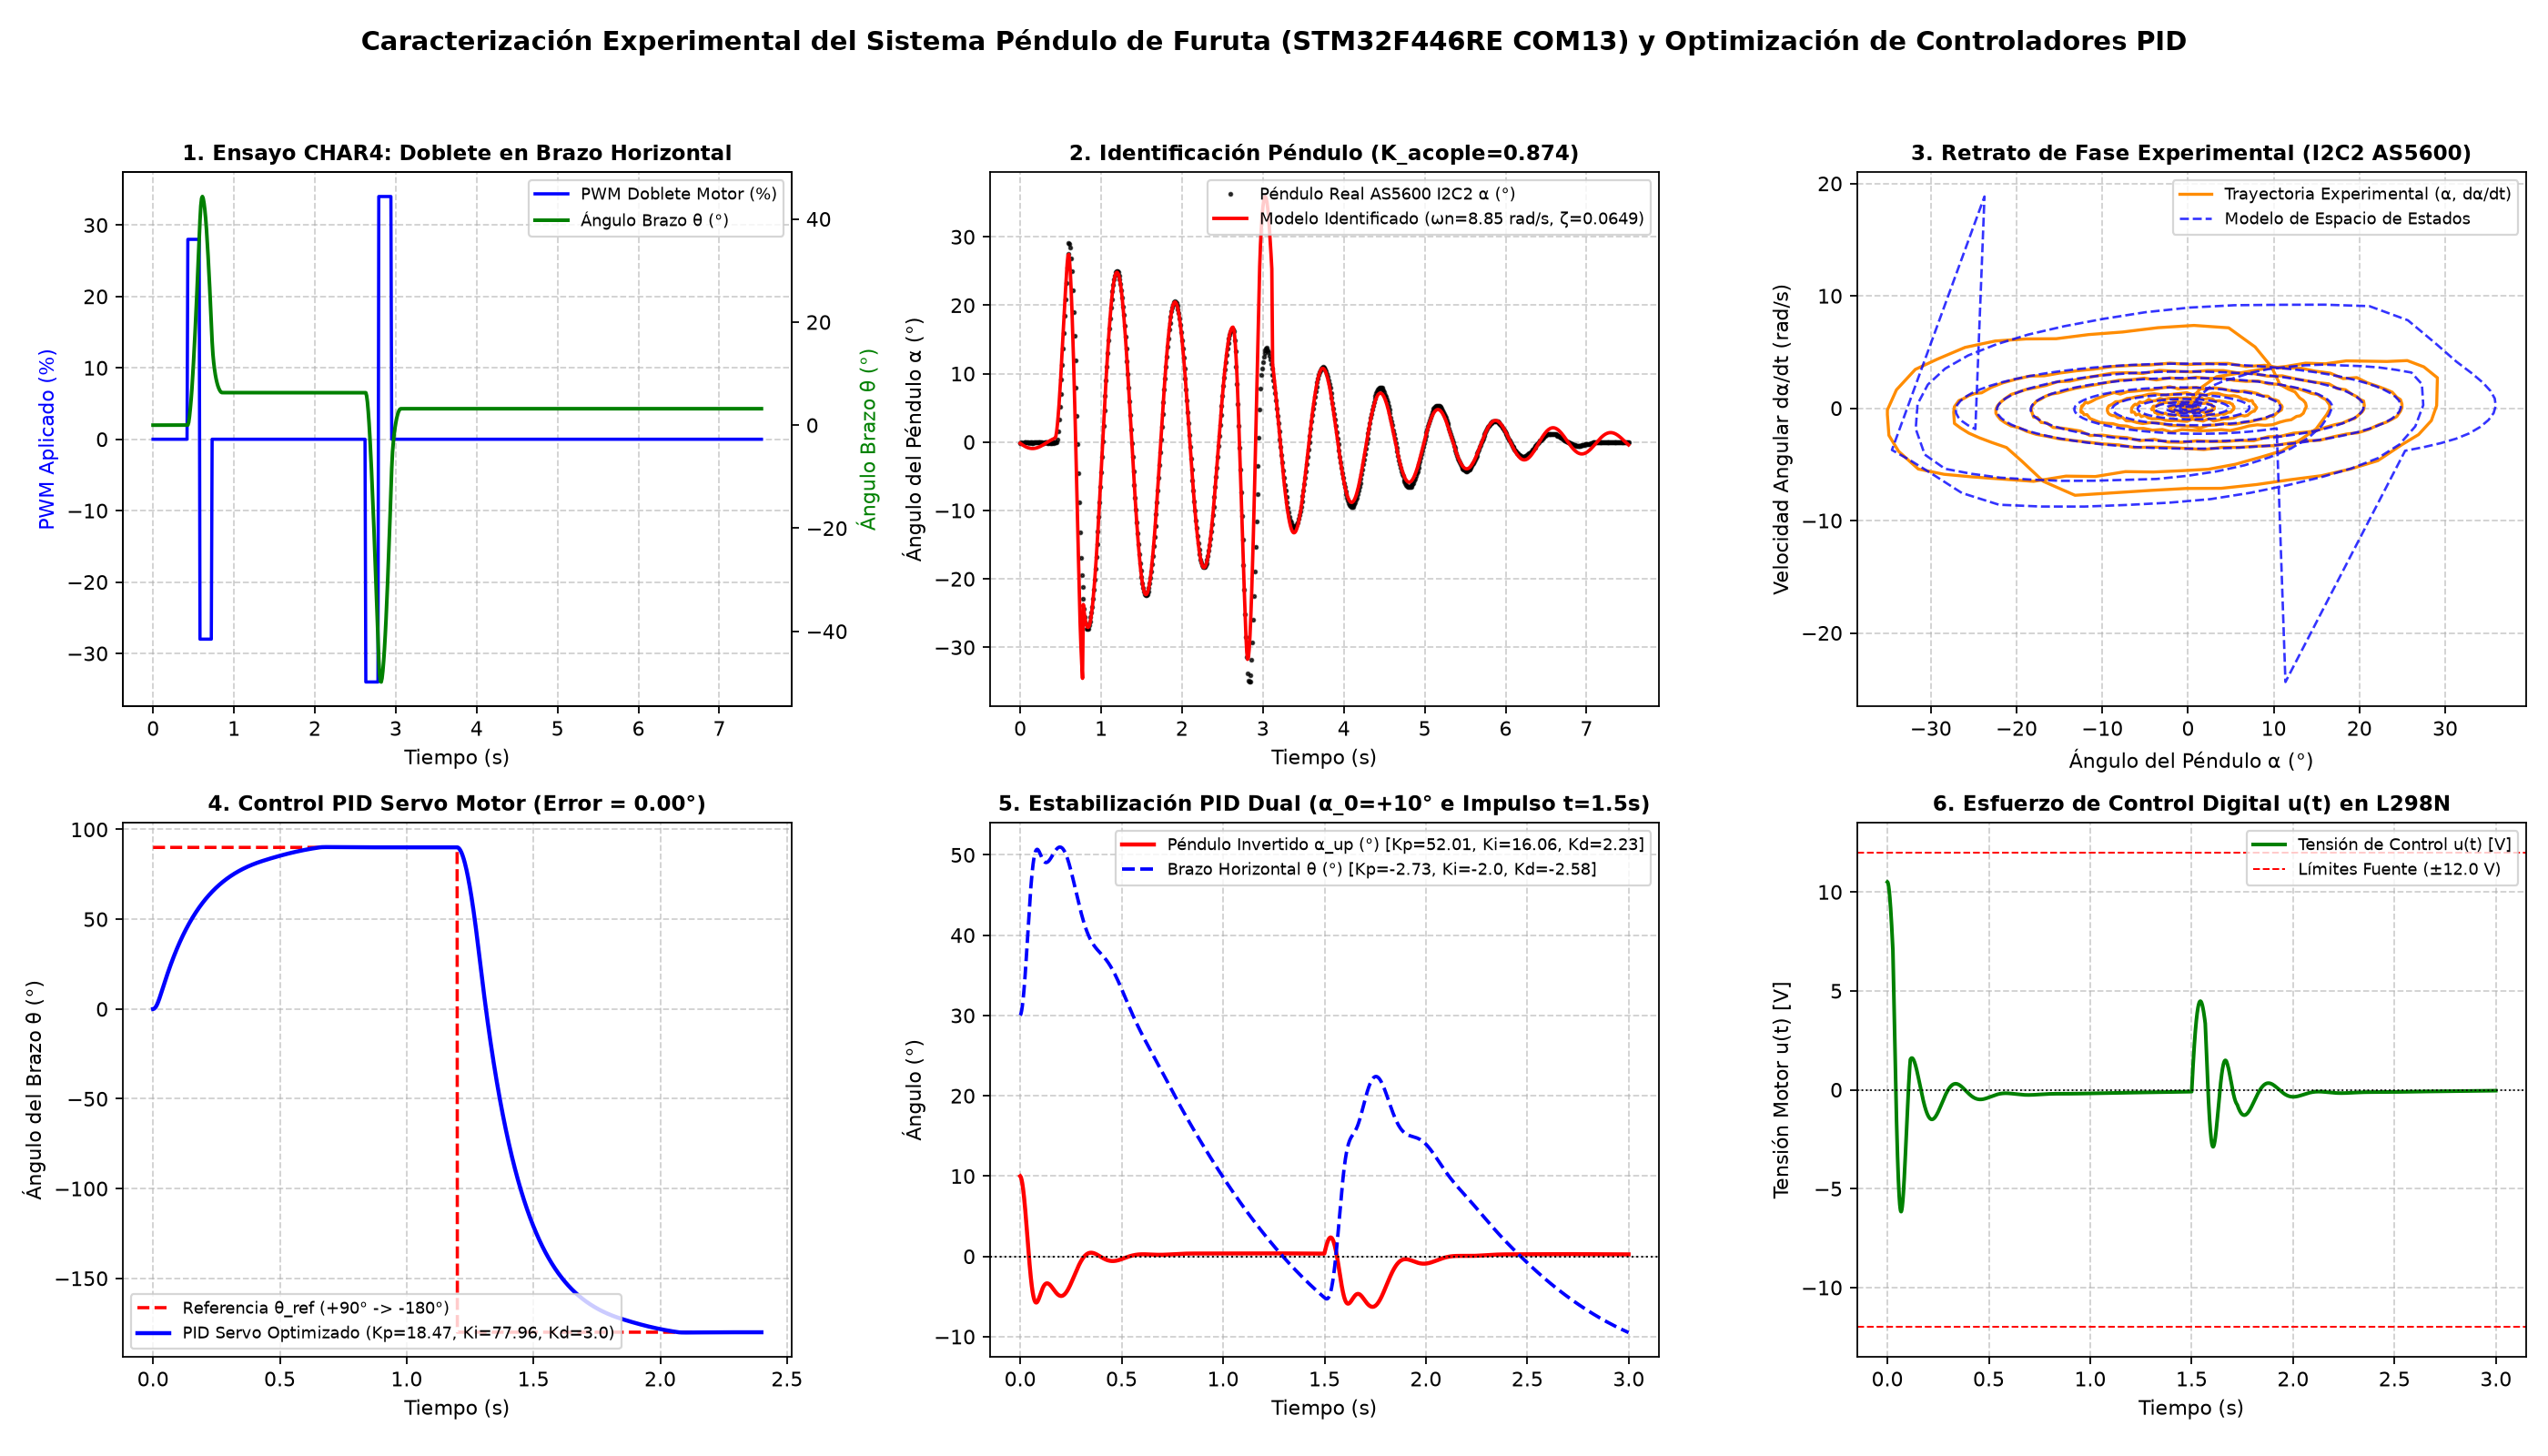
\includegraphics[width=0.80\textwidth]{fig_exp_caracterizacion_sistema.png}
    \caption{Identificación CHAR4 ($768$ muestras) y optimización PID: doblete con freno activo, ajuste $\omega_n=\qty{8.85}{\radian\per\second}$ ($\zeta=0.0649$, $K_{\text{acople}}=0.874$), retrato de fase y validación simulada.}
    \label{fig:exp_sistema}
\end{figure*}

\subsection{Firmware, Estrategia M4 Ultra-Silk y Gemelo Digital 3D}\label{subsec:firmware_control}
El firmware se estructura en cinco capas desacopladas (Fig.~\ref{fig:arquitectura_firmware}): \texttt{DMA1\_Stream5} RX circular (\qty{128}{\byte} a \qty{115200}{\baud}) captura comandos sin bloquear \texttt{TIM6}, y el superlazo emite telemetría CSV de 9 canales a \qty{100}{\hertz}. La FSM (Fig.~\ref{fig:fsm_firmware}) inicia en \texttt{IDLE=0}, lanza \texttt{SWING\_UP=5} con \texttt{START}, conmuta a \texttt{BALANCE\_PID=6} sin límite angular $\theta$, ejecuta auto-recuperación en \texttt{RECOVER\_HOME=8} si $|\tilde{\alpha}|>32^\circ$ y aparca en $\qty{0}{\degree}$ con \texttt{STOP\_HOME=9}.

\begin{figure*}[!t]
\centering
\definecolor{archApp}{HTML}{E8F0FE}
\definecolor{archAppBorder}{HTML}{1A73E8}
\definecolor{archComm}{HTML}{FEF7E0}
\definecolor{archCommBorder}{HTML}{F9AB00}
\definecolor{archDrv}{HTML}{E6F4EA}
\definecolor{archDrvBorder}{HTML}{137333}
\definecolor{archHal}{HTML}{FCE8E6}
\definecolor{archHalBorder}{HTML}{C5221F}
\definecolor{archHw}{HTML}{F1F3F4}
\definecolor{archHwBorder}{HTML}{5F6368}
\definecolor{archText}{HTML}{202124}

\def\colGapFour{0.36cm}
\def\titleDrop{-1.10cm}
\def\subDrop{-0.20cm}

\resizebox{0.94\textwidth}{!}{%
\begin{tikzpicture}[
    >=Stealth,
    font=\small,
    layerbox/.style={
        rectangle, rounded corners=5pt, draw=#1, line width=1.15pt,
        fill=#1!10, inner xsep=0.35cm, inner ysep=0.28cm
    },
    layertitle/.style={
        font=\small\bfseries, inner sep=1pt
    },
    subblock/.style={
        rectangle, rounded corners=3pt, draw=#1!80!black, line width=0.65pt,
        fill=white, font=\scriptsize, align=center, inner xsep=4pt, inner ysep=5pt,
        minimum height=1.55cm
    },
    flow/.style={<->, >={Stealth[length=4.5pt, width=3.8pt]}, thick, color=archText!70}
]

% ==================== CAPA 5 (Referencia maestra superior) ====================
\node[layertitle, text=archAppBorder] (L5t)
    {Capa 5: Algoritmos de Control Digital y FSM (\texttt{furuta\_control.c / pid\_controller.c})};

\node[subblock=archAppBorder, minimum height=1.72cm, text width=4.00cm, anchor=north west] (b1)
    at ($(L5t.south west)+(0,\subDrop)$)
    {\textbf{FSM 10 Estados Determinista}\\\texttt{IDLE}, \texttt{SWING\_UP},\\\texttt{BALANCE\_PID}, \texttt{RECOVER}, \texttt{STOP}};
\node[subblock=archAppBorder, minimum height=1.72cm, text width=4.40cm, right=\colGapFour of b1.north east, anchor=north west] (b2)
    {\textbf{Lazo Dual M4 Ultra-Silk}\\$K_{p,\alpha}=14.5,\; K_{d,\alpha}=1.5$\\$K_{p,\theta}=-1.45,\; K_{i,\theta}=-0.75$\\$K_{d,\theta}=-0.85$};
\node[subblock=archAppBorder, minimum height=1.72cm, text width=3.80cm, right=\colGapFour of b2.north east, anchor=north west] (b3)
    {\textbf{Filtros Dual-Notch Biquad}\\Fijo: \qty{11.0}{\hertz} ($Q=1.2$)\\Adap.: \qty{6.2}{\hertz} ($-6\text{ dB}, Q=1.4$)};
\node[subblock=archAppBorder, minimum height=1.72cm, text width=3.80cm, right=\colGapFour of b3.north east, anchor=north west] (b4)
    {\textbf{Swing-Up y Servo Clegg}\\Bombeo $E_{\text{norm}}$ ($\omega_n=8.85$)\\Clegg Reset + \texttt{L298N\_Brake}};

\coordinate (row_w) at (b1.west);
\coordinate (row_e) at (b4.east);
\coordinate (row5_w) at (row_w |- b1.center);
\coordinate (row5_e) at (row_e |- b1.center);

\begin{scope}[on background layer]
    \node[layerbox=archAppBorder, fit=(L5t)(b1)(b2)(b3)(b4)(row5_w)(row5_e)] (L5) {};
\end{scope}

% ==================== CAPA 4 ====================
\node[layertitle, text=archCommBorder!90!black, anchor=north west] (L4t)
    at ($(row_w |- L5.south)+(0,\titleDrop)$)
    {Capa 4: Comunicaci\'on Serial y Telemetr\'ia (\texttt{main.c / stm32f4xx\_it.c})};

\node[subblock=archCommBorder, text width=5.51cm, anchor=north west] (c1)
    at ($(row_w |- L4t.south)+(0,\subDrop)$)
    {\textbf{UART DMA1\_S5 Circular (\texttt{USART2})}\\B\'ufer RX \qty{128}{\byte} a \qty{115200}{\baud}\\0\% p\'erdida sin bloquear lazo de \qty{1}{\kilo\hertz}};
\node[subblock=archCommBorder, text width=5.51cm, anchor=north east] (c3)
    at (row_e |- c1.north)
    {\textbf{Telemetr\'ia CSV Decimada @ \qty{100}{\hertz}}\\Env\'io cada \qty{10}{\milli\second} (\texttt{DECM=10})\\9 canales: $t, \text{est}, \text{pwm}, u, \theta, \omega, \alpha, \tilde{\alpha}, \dot{\alpha}$};
\node[subblock=archCommBorder, text width=5.51cm, anchor=north] (c2)
    at ($(c1.north east)!0.5!(c3.north west)$)
    {\textbf{Parser As\'incrono de Comandos}\\Comandos \texttt{START}, \texttt{STOPHOME}, \texttt{ZERO}, \texttt{CHAR*}\\Decodificaci\'on en superloop de fondo};

\coordinate (row4_w) at (row_w |- c1.center);
\coordinate (row4_e) at (row_e |- c1.center);

\begin{scope}[on background layer]
    \node[layerbox=archCommBorder, fit=(L4t)(c1)(c2)(c3)(row4_w)(row4_e)] (L4) {};
\end{scope}

% ==================== CAPA 3 ====================
\node[layertitle, text=archDrvBorder, anchor=north west] (L3t)
    at ($(row_w |- L4.south)+(0,\titleDrop)$)
    {Capa 3: Drivers de Dispositivos y Sensado (\texttt{as5600.c / l298n\_motor.c})};

\node[subblock=archDrvBorder, text width=5.51cm, anchor=north west] (d1)
    at ($(row_w |- L3t.south)+(0,\subDrop)$)
    {\textbf{Doble Bus Soft-$\text{I}^2\text{C}$ ($\sim\qty{450}{\kilo\hertz}$)}\\Buses \texttt{PB8/PB9} ($\theta$) y \texttt{PB10/PB3} ($\alpha$)\\Auto-detecci\'on SCL/SDA en $< \qty{45}{\micro\second}$};
\node[subblock=archDrvBorder, text width=5.51cm, anchor=north east] (d3)
    at (row_e |- d1.north)
    {\textbf{Driver Puente H L298N}\\Comp.\ suave $+9.2\%/-16.0\%$ ($V_k=\qty{0.65}{\volt}$)\\Espejos redundantes \texttt{PA9/PA10} en \texttt{IN2}};
\node[subblock=archDrvBorder, text width=5.51cm, anchor=north] (d2)
    at ($(d1.north east)!0.5!(d3.north west)$)
    {\textbf{Procesamiento AS5600}\\Desenvolvimiento multi-vuelta ($80{:}1$)\\LPF IIR velocidad ($\tau=\qty{6}{\milli\second}$)};

\coordinate (row3_w) at (row_w |- d1.center);
\coordinate (row3_e) at (row_e |- d1.center);

\begin{scope}[on background layer]
    \node[layerbox=archDrvBorder, fit=(L3t)(d1)(d2)(d3)(row3_w)(row3_e)] (L3) {};
\end{scope}

% ==================== CAPA 2 ====================
\node[layertitle, text=archHalBorder, anchor=north west] (L2t)
    at ($(row_w |- L3.south)+(0,\titleDrop)$)
    {Capa 2: Abstracci\'on de Hardware, Timers e Interrupciones (STM32 HAL / CMSIS)};

\node[subblock=archHalBorder, text width=5.51cm, anchor=north west] (h1)
    at ($(row_w |- L2t.south)+(0,\subDrop)$)
    {\textbf{Temporizador \texttt{TIM6} @ \qty{1.0}{\kilo\hertz}}\\Clock \qty{90}{\mega\hertz} (\texttt{PSC=89, ARR=999})\\Interrupci\'on NVIC Prioridad 1};
\node[subblock=archHalBorder, text width=5.51cm, anchor=north east] (h3)
    at (row_e |- h1.north)
    {\textbf{Controlador \texttt{DMA1\_Stream5} (Ch4)}\\Transferencia directa \texttt{USART2->DR}\\Interrupci\'on EXTI B1 (\texttt{PC13})};
\node[subblock=archHalBorder, text width=5.51cm, anchor=north] (h2)
    at ($(h1.north east)!0.5!(h3.north west)$)
    {\textbf{Generador PWM \texttt{TIM1\_CH1} (\texttt{PA8})}\\Clock \qty{180}{\mega\hertz} (\texttt{PSC=9, ARR=899})\\Portadora ultras\'onica \qty{20.0}{\kilo\hertz} ($0\text{--}900$)};

\coordinate (row2_w) at (row_w |- h1.center);
\coordinate (row2_e) at (row_e |- h1.center);

\begin{scope}[on background layer]
    \node[layerbox=archHalBorder, fit=(L2t)(h1)(h2)(h3)(row2_w)(row2_e)] (L2) {};
\end{scope}

% ==================== CAPA 1 ====================
\node[layertitle, text=archHwBorder!90!black, anchor=north west] (L1t)
    at ($(row_w |- L2.south)+(0,\titleDrop)$)
    {Capa 1: Plataforma F\'isica y Microcontrolador STM32F446RET6};

\node[subblock=archHwBorder, text width=4.00cm, anchor=north west] (w1)
    at ($(row_w |- L1t.south)+(0,\subDrop)$)
    {\textbf{ARM Cortex-M4F}\\HSE \qty{8}{\mega\hertz} $\rightarrow$ PLL \qty{180}{\mega\hertz}\\FPU hardware activa (FPv4-SP)};
\node[subblock=archHwBorder, text width=4.00cm, right=\colGapFour of w1.north east, anchor=north west] (w2)
    {\textbf{Memoria y Aceleraci\'on}\\Flash \qty{512}{\kilo\byte} (ART, 5 WS)\\SRAM \qty{128}{\kilo\byte} (B\'ufer/Estado)};
\node[subblock=archHwBorder, text width=4.00cm, right=\colGapFour of w2.north east, anchor=north west] (w3)
    {\textbf{Potencia L298N + Motor}\\Fuente \qty{12}{\volt} DC · Namiki 80:1\\Diodos r\'apidos Flyback};
\node[subblock=archHwBorder, text width=4.00cm, right=\colGapFour of w3.north east, anchor=north west] (w4)
    {\textbf{Sensores AS5600 (2$\times$)}\\Efecto Hall 12 bits (\texttt{0x36})\\$\qty{0.0879}{\degree}$ distal · $\qty{0.0011}{\degree}$ motor};

\coordinate (row1_w) at (row_w |- w1.center);
\coordinate (row1_e) at (row_e |- w1.center);

\begin{scope}[on background layer]
    \node[layerbox=archHwBorder, fit=(L1t)(w1)(w2)(w3)(w4)(row1_w)(row1_e)] (L1) {};
\end{scope}

% ==================== FLUJOS VERTICALES ENTRE CAPAS ====================
\draw[flow] (L5.south) -- (L4.north) node[midway, right=6pt, font=\scriptsize, text=archText!75] {Comandos / Telemetr\'ia};
\draw[flow] (L4.south) -- (L3.north) node[midway, right=6pt, font=\scriptsize, text=archText!75] {Lecturas $\theta,\alpha$ / Voltaje $u$};
\draw[flow] (L3.south) -- (L2.north) node[midway, right=6pt, font=\scriptsize, text=archText!75] {Registros GPIO / TIM};
\draw[flow] (L2.south) -- (L1.north) node[midway, right=6pt, font=\scriptsize, text=archText!75] {Se\~nales el\'ectricas f\'isicas};

\end{tikzpicture}%
}
\caption{Arquitectura modular en cinco capas del firmware embebido sobre STM32 Nucleo-F446RE, desacoplando el lazo is\'ocrono de control (\texttt{TIM6} a \qty{1.0}{\kilo\hertz}) de la comunicaci\'on UART por hardware DMA (\qty{100}{\hertz}) y los controladores Soft-$\text{I}^2\text{C}$ / PWM (\qty{20.0}{\kilo\hertz}).}
\label{fig:arquitectura_firmware}
\end{figure*}

% ==============================================================================
% Figura 5: Máquina de Estados Finitos (FSM) del Firmware furuta_control.c (1 kHz)
% Diseño por construcción (Layout by Construction): posicionamiento relativo,
% anclas exactas, contenedores elásticos (fit) y cero cruces de transiciones.
% Bibliotecas TikZ requeridas: arrows.meta, positioning, fit, calc.
% ==============================================================================
\begin{figure*}[!t]
\centering
\resizebox{\textwidth}{!}{%
\begin{tikzpicture}[
    font=\sffamily,
    % --- Paleta semántica suave (ámbito local al entorno tikzpicture) ---
    /utils/exec={%
        \definecolor{fsmIdleFill}{HTML}{F1F5F9}%
        \definecolor{fsmIdleBdr}{HTML}{475569}%
        \definecolor{fsmIdleHdr}{HTML}{334155}%
        \definecolor{fsmServFill}{HTML}{EFF6FF}%
        \definecolor{fsmServBdr}{HTML}{2563EB}%
        \definecolor{fsmServHdr}{HTML}{1D4ED8}%
        \definecolor{fsmServZoneBdr}{HTML}{60A5FA}%
        \definecolor{fsmServZonePill}{HTML}{DBEAFE}%
        \definecolor{fsmServZoneTxt}{HTML}{1E3A8A}%
        \definecolor{fsmWarmFill}{HTML}{FFF7ED}%
        \definecolor{fsmWarmBdr}{HTML}{EA580C}%
        \definecolor{fsmWarmHdr}{HTML}{C2410C}%
        \definecolor{fsmWarmSubFill}{HTML}{FFEDD5}%
        \definecolor{fsmWarmSubBdr}{HTML}{FB923C}%
        \definecolor{fsmHeroFill}{HTML}{ECFDF5}%
        \definecolor{fsmHeroBdr}{HTML}{059669}%
        \definecolor{fsmHeroHdr}{HTML}{047857}%
        \definecolor{fsmAutoZoneBdr}{HTML}{0D9488}%
        \definecolor{fsmAutoZonePill}{HTML}{CCFBF1}%
        \definecolor{fsmAutoZoneTxt}{HTML}{115E59}%
        \definecolor{fsmStopFill}{HTML}{FEF2F2}%
        \definecolor{fsmStopBdr}{HTML}{DC2626}%
        \definecolor{fsmStopHdr}{HTML}{B91C1C}%
        \definecolor{fsmAlertFill}{HTML}{FFF1F2}%
        \definecolor{fsmAlertBdr}{HTML}{E11D48}%
        \definecolor{fsmAlertTxt}{HTML}{9F1239}%
        \definecolor{fsmInk}{HTML}{1E293B}%
        \definecolor{fsmMuted}{HTML}{475569}%
    },
    % --- Estilos de nodos de estado (Layout by Construction) ---
    fsmNode/.style={
        rectangle,
        rounded corners=8pt,
        align=center,
        inner xsep=7pt,
        inner ysep=6pt,
        text=fsmInk,
        line width=1.0pt
    },
    stateIdle/.style={
        fsmNode,
        fill=fsmIdleFill,
        draw=fsmIdleBdr,
        line width=1.25pt,
        text width=3.95cm,
        minimum height=2.40cm
    },
    stateServ/.style={
        fsmNode,
        fill=fsmServFill,
        draw=fsmServBdr,
        text width=4.40cm,
        minimum height=1.65cm
    },
    stateSwing/.style={
        fsmNode,
        fill=fsmWarmFill,
        draw=fsmWarmBdr,
        line width=1.1pt,
        text width=4.75cm,
        minimum height=2.35cm
    },
    stateHero/.style={
        fsmNode,
        fill=fsmHeroFill,
        draw=fsmHeroBdr,
        line width=1.75pt,
        text width=5.25cm,
        minimum height=2.35cm
    },
    stateRecover/.style={
        fsmNode,
        fill=fsmWarmFill,
        draw=fsmWarmBdr,
        line width=1.1pt,
        text width=11.4cm,
        minimum height=2.05cm
    },
    stateStop/.style={
        fsmNode,
        fill=fsmStopFill,
        draw=fsmStopBdr,
        line width=1.1pt,
        text width=8.2cm,
        minimum height=1.40cm
    },
    % --- Estilos de transiciones (flechas canónicas) ---
    transMain/.style={
        -{Stealth[length=2.7mm, width=1.95mm]},
        line width=1.15pt,
        draw=fsmAutoZoneTxt,
        shorten >=1.5pt,
        shorten <=1.0pt
    },
    transWarm/.style={
        -{Stealth[length=2.7mm, width=1.95mm]},
        line width=1.15pt,
        draw=fsmWarmHdr,
        shorten >=1.5pt,
        shorten <=1.0pt
    },
    transServ/.style={
        -{Stealth[length=2.3mm, width=1.7mm]},
        line width=0.95pt,
        draw=fsmServHdr,
        shorten >=1.5pt,
        shorten <=1.0pt
    },
    transRet/.style={
        -{Stealth[length=2.3mm, width=1.7mm]},
        line width=0.90pt,
        draw=fsmIdleBdr,
        shorten >=1.5pt,
        shorten <=1.0pt
    },
    transBypass/.style={
        -{Stealth[length=2.5mm, width=1.8mm]},
        line width=1.05pt,
        draw=fsmHeroHdr,
        dashed,
        dash pattern=on 5pt off 3pt,
        shorten >=1.5pt,
        shorten <=1.0pt
    },
    transStop/.style={
        -{Stealth[length=2.6mm, width=1.9mm]},
        line width=1.1pt,
        draw=fsmStopHdr,
        shorten >=1.5pt,
        shorten <=1.0pt
    },
    % --- Etiquetas de transición ---
    elbl/.style={
        font=\small\sffamily,
        text=fsmInk,
        align=center,
        inner sep=1.8pt
    },
    elblBox/.style={
        elbl,
        fill=white,
        rounded corners=2pt,
        inner xsep=3.5pt,
        inner ysep=2pt
    },
    % --- Badges y contenedores ---
    zoneServ/.style={
        draw=fsmServZoneBdr,
        dashed,
        line width=0.95pt,
        rounded corners=10pt,
        fill=none,
        inner xsep=0.34cm,
        inner ysep=0.45cm
    },
    zoneAuto/.style={
        draw=fsmAutoZoneBdr,
        dashed,
        line width=1.1pt,
        rounded corners=10pt,
        fill=none,
        inner xsep=0.36cm,
        inner ysep=0.50cm
    },
    zonePill/.style={
        rectangle,
        rounded corners=3.5pt,
        font=\small\bfseries\sffamily,
        inner xsep=6pt,
        inner ysep=2.5pt
    }
]

% ==============================================================================
% 1. COLOCACIÓN RELATIVA DE ESTADOS (LAYOUT BY CONSTRUCTION)
% ==============================================================================

% --- Núcleo central: Estado Inicial IDLE (Estado 0) ---
\node[stateIdle] (idle) at (0,0) {%
    \colorbox{fsmIdleHdr}{\textcolor{white}{\footnotesize\bfseries Est.\,0}}\\[3pt]
    {\large\bfseries IDLE}\\[2pt]
    {\small Estado inicial / reposo}\\
    {\small Rueda libre (\texttt{L298N\_Coast})}\\
    {\small \mbox{$u = \qty{0}{\volt}$}}
};

% --- Rama Izquierda: Servicio y Diagnóstico (Estados 1, 2, 3–4) ---
\node[stateServ, left=3.75cm of idle] (char) {%
    \colorbox{fsmServHdr}{\textcolor{white}{\footnotesize\bfseries Est.\,2}}\\[3pt]
    {\normalsize\bfseries CHARACTERIZATION}\\[2pt]
    {\small Ensayos \texttt{CHAR1}--\texttt{CHAR4}}\\
    {\small Validaci\'on PID (\texttt{CHAR5A/B})}
};

\node[stateServ, above=0.95cm of char] (cal) {%
    \colorbox{fsmServHdr}{\textcolor{white}{\footnotesize\bfseries Est.\,1}}\\[3pt]
    {\normalsize\bfseries CALIBRATING}\\[2pt]
    {\small Promedio de 64 muestras}\\
    {\small Cero de encoders AS5600}
};

\node[stateServ, below=0.95cm of char] (pidmp) {%
    \colorbox{fsmServHdr}{\textcolor{white}{\footnotesize\bfseries Est.\,3--4}}\\[3pt]
    {\small\bfseries MOTOR\_PID\_VEL / POS}\\[2pt]
    {\small PID Tustin (vel.) / Servo}\\
    {\small Clegg + freno activo}
};

% --- Rama Principal Derecha: Ciclo Autónomo de Control Furuta ---
% Fila superior del ciclo: SWING_UP (Est. 5) y BALANCE_PID (Est. 6, HERO)
\node[stateSwing, right=3.80cm of idle, yshift=1.70cm] (swing) {%
    \colorbox{fsmWarmHdr}{\textcolor{white}{\footnotesize\bfseries Est.\,5}}\\[3pt]
    {\large\bfseries SWING\_UP}\\[2pt]
    {\small Bombeo resonante\\en cuadratura}\\
    {\small Carrera adaptativa: $50^\circ / 36^\circ / 22^\circ$}
};

\node[stateHero, right=2.90cm of swing] (balance) {%
    \colorbox{fsmHeroHdr}{\textcolor{white}{\footnotesize\bfseries Est.\,6 \;$\bullet$\; EQUILIBRIO}}\\[3pt]
    {\large\bfseries\color{fsmHeroHdr} BALANCE\_PID}\\[2pt]
    {\small M4 Ultra-Silk + Dual-Notch\\(\qty{11}{\hertz} / \qty{6.2}{\hertz})}\\
    {\small Slew adaptativo; sin límite angular $\theta$}
};

% Fila inferior del ciclo: RECOVER_HOME (Est. 8) centrado bajo SWING_UP y BALANCE_PID
\coordinate (auto_row1_mid) at ($(swing.south west)!0.5!(balance.south east)$);
\node[stateRecover, anchor=north] (recover) at ($(auto_row1_mid)+(0,-1.95cm)$) {%
    \colorbox{fsmWarmHdr}{\textcolor{white}{\footnotesize\bfseries Est.\,8}}\quad
    {\large\bfseries RECOVER\_HOME}\quad
    {\small (Auto-recuperación en 3 subfases)}\\[5pt]
    \fcolorbox{fsmWarmSubBdr}{fsmWarmSubFill}{\small\strut\textbf{F0:} Rueda libre (\qty{300}{\milli\second})}%
    \;\mbox{$\rightarrow$}\;%
    \fcolorbox{fsmWarmSubBdr}{fsmWarmSubFill}{\small\strut\textbf{F1:} Retorno suave a $\theta = 0^\circ$}\\[4pt]%
    \mbox{$\rightarrow$}\;%
    \fcolorbox{fsmWarmSubBdr}{fsmWarmSubFill}{\small\strut\textbf{F2:} Freno activo hasta calma (\qty{250}{\milli\second})}
};

% ==============================================================================
% 2. CONTENEDORES ELÁSTICOS (FIT) CON ENCABEZADOS TIPO PILL
% ==============================================================================

% Contenedor Zona Servicio y Diagnóstico
\coordinate (serv_top_pad) at ($(cal.north)+(0,0.20cm)$);
\node[zoneServ, fit=(cal)(char)(pidmp)(serv_top_pad)] (serv_zone) {};
\node[zonePill, fill=fsmServZonePill, draw=fsmServZoneBdr, text=fsmServZoneTxt]
    at (serv_zone.north) {Servicio y Diagnóstico};

% Contenedor Superestado Ciclo Autónomo Cerrado
\coordinate (auto_top_pad) at ($(swing.north)+(0,0.30cm)$);
\node[zoneAuto, fit=(swing)(balance)(recover)(auto_top_pad)] (auto_zone) {};
\node[zonePill, fill=fsmAutoZonePill, draw=fsmAutoZoneBdr, text=fsmAutoZoneTxt, anchor=west]
    at ([xshift=0.35cm]auto_zone.north west) {Ciclo Autónomo Cerrado de Control Furuta};

% --- Parada Ordenada: STOP_HOME (Est. 9) bajo el superestado autónomo ---
\node[stateStop, below=1.10cm of auto_zone.south] (stophome) {%
    \colorbox{fsmStopHdr}{\textcolor{white}{\footnotesize\bfseries Est.\,9}}\quad
    {\large\bfseries STOP\_HOME}\\[3pt]
    {\small Parada ordenada (botón \textbf{Detener} MATLAB):\\retorno suave a \mbox{$\theta = 0^\circ$} y paso a \texttt{IDLE}}
};

% ==============================================================================
% 3. TRANSICIONES Y ETIQUETAS (CERO CRUCES, ANCLAS EXACTAS)
% ==============================================================================

% --- Entrada inicial a IDLE (Inicio / ISR 1 kHz) ---
\coordinate (init_dot) at ([xshift=-0.70cm, yshift=0.95cm]idle.north);
\fill[fsmIdleHdr] (init_dot) circle (3.2pt);
\draw[transRet, line width=1.15pt, draw=fsmIdleHdr]
    (init_dot) -- ([xshift=-0.70cm]idle.north);
\node[elbl, above=2.5pt] at (init_dot) {\textbf{Reset / Inicio}\\ISR $\qty{1}{\kilo\hertz}$};

% --- Carriles de ruteo ortogonal en la brecha izquierda (Service <-> IDLE) ---
\coordinate (laneL_near_idle) at ($(idle.west)+(-0.38cm,0)$);
\coordinate (laneL_mid)       at ($(idle.west)+(-0.76cm,0)$);
\coordinate (gapL_mid_near)   at ($(serv_zone.east)!0.5!(laneL_near_idle)$);
\coordinate (gapL_mid_lane)   at ($(serv_zone.east)!0.5!(laneL_mid)$);

% IDLE -> CALIBRATING (ZERO / Botón B1)
\coordinate (cal_in)  at ([yshift=0.22cm]cal.east);
\coordinate (cal_out) at ([yshift=-0.22cm]cal.east);
\draw[transServ, rounded corners=6pt]
    ([yshift=0.88cm]idle.west) -- ([yshift=0.88cm]idle.west -| laneL_near_idle)
    -- (cal_in -| laneL_near_idle)
    -- (cal_in);
\node[elbl, above=2pt] at (cal_in -| gapL_mid_near) {\texttt{ZERO} / Botón B1};

% CALIBRATING -> IDLE (Calibración completa)
\draw[transRet, rounded corners=6pt]
    (cal_out) -- (cal_out -| laneL_mid)
    -- ([yshift=0.58cm]idle.west -| laneL_mid)
    -- ([yshift=0.58cm]idle.west);
\node[elbl, below=2pt, text=fsmMuted] at (cal_out -| gapL_mid_lane) {Calibrado};

% IDLE <-> CHARACTERIZATION (paralelas rectas)
\draw[transServ]
    ([yshift=0.20cm]idle.west) -- ([yshift=0.20cm]char.east);
\node[elbl, above=2pt] at ([yshift=0.20cm]gapL_mid_lane) {\texttt{CHAR1}--\texttt{CHAR5}};
\draw[transRet]
    ([yshift=-0.20cm]char.east) -- ([yshift=-0.20cm]idle.west);
\node[elbl, below=2pt, text=fsmMuted] at ([yshift=-0.20cm]gapL_mid_lane) {\texttt{test\_finished}};

% IDLE -> MOTOR_PID_VEL / POS
\draw[transServ, rounded corners=6pt]
    ([yshift=-0.82cm]idle.west) -- ([yshift=-0.82cm]idle.west -| laneL_near_idle)
    -- (pidmp.east -| laneL_near_idle)
    -- (pidmp.east);
\node[elbl, above=2pt] at (pidmp.east -| gapL_mid_near) {\texttt{VEL=} / \texttt{POS=}};

% --- Carril de ruteo derecho (IDLE -> Ciclo Autónomo) ---
\coordinate (laneR_near_idle) at ($(idle.east)+(0.42cm,0)$);
\coordinate (gapR_mid)        at ($(laneR_near_idle)!0.5!(auto_zone.west)$);

% IDLE -> SWING_UP (START/SWING si está en 0° y reposo)
\draw[transMain, rounded corners=6pt]
    ([yshift=0.65cm]idle.east) -- ([yshift=0.65cm]idle.east -| laneR_near_idle)
    -- (swing.west -| laneR_near_idle)
    -- (swing.west);
\node[elbl, above=2pt] at (swing.west -| gapR_mid) {\texttt{START} / \texttt{SWING}};
\node[elbl, below=2pt, text=fsmMuted] at (swing.west -| gapR_mid) {(en $0^\circ$ y reposo)};

% IDLE -> RECOVER_HOME (START/SWING si brazo != 0° o en movimiento)
\draw[transWarm, rounded corners=6pt]
    ([yshift=-0.65cm]idle.east) -- ([yshift=-0.65cm]idle.east -| laneR_near_idle)
    -- (recover.west -| laneR_near_idle)
    -- (recover.west);
\node[elbl, above=2pt] at (recover.west -| gapR_mid) {\texttt{START} / \texttt{SWING}};
\node[elbl, below=2pt, text=fsmMuted] at (recover.west -| gapR_mid) {($\theta \neq 0^\circ$ o mov.)};

% IDLE -> BALANCE_PID (acceso directo por corredor superior, cero cruces)
\coordinate (top_rail) at ($(auto_zone.north)+(0,0.75cm)$);
\coordinate (bal_exit) at ([xshift=0.70cm]idle.north);
\draw[transBypass, rounded corners=7pt]
    (bal_exit) -- (bal_exit |- top_rail)
    -- node[pos=0.55, above=2pt, elbl, text=fsmHeroHdr]
       {\texttt{BALANCE} \;{\color{fsmMuted}(acceso directo, \texttt{auto\_swingup=false})}}
       (balance.north |- top_rail)
    -- (balance.north);

% --- Transiciones internas del Ciclo Autónomo Cerrado ---

% SWING_UP -> BALANCE_PID (Transferencia sin saltos / bumpless)
\draw[transMain, draw=fsmHeroHdr, line width=1.35pt]
    (swing.east) --
    node[above=3pt, elbl] {$|\tilde{\alpha}| < 20^\circ$\\$|\dot{\alpha}| < \qty{4.8}{\radian\per\second}$}
    node[below=3pt, elbl, text=fsmHeroHdr] {\bfseries Transferencia\\[-1pt]\bfseries sin saltos}
    (balance.west);

% SWING_UP -> RECOVER_HOME (Timeout > 5.5 s)
\coordinate (sw_tmo_top) at ([xshift=-1.15cm]swing.south);
\coordinate (sw_tmo_bot) at (sw_tmo_top |- recover.north);
\draw[transWarm]
    (sw_tmo_top) -- node[pos=0.50, elblBox, text=fsmWarmHdr] {Timeout\\$t > \qty{5.5}{\second}$} (sw_tmo_bot);

% RECOVER_HOME -> SWING_UP (Relanza automáticamente SWING_UP — ciclo cerrado)
\coordinate (sw_rel_top) at ([xshift=1.05cm]swing.south);
\coordinate (sw_rel_bot) at (sw_rel_top |- recover.north);
\draw[transMain, line width=1.25pt]
    (sw_rel_bot) -- node[pos=0.50, right=4pt, elbl, align=left, text=fsmAutoZoneTxt]
        {\textbf{Ciclo cerrado}\\Calma $\qty{250}{\milli\second}$\\$\rightarrow$ relanza \texttt{SWING\_UP}} (sw_rel_top);

% BALANCE_PID -> RECOVER_HOME (Watchdog de caída |alpha_tilde| > 32° y auto_swingup=true)
\coordinate (bal_wd_bot) at (balance.south |- recover.north);
\draw[transWarm, line width=1.25pt]
    (balance.south) -- node[pos=0.50, elblBox, text=fsmWarmHdr]
        {\textbf{Watchdog caída}\\$|\tilde{\alpha}| > 32^\circ \land \texttt{auto\_swingup=true}$} (bal_wd_bot);

% --- Parada ordenada: Ciclo Autónomo -> STOP_HOME -> IDLE ---
\draw[transStop]
    (auto_zone.south) -- node[midway, right=5pt, elbl, align=left, text=fsmStopHdr]
        {\texttt{STOPHOME} {\color{fsmMuted}(desde ciclo autónomo)}} (stophome.north);

\draw[transStop, rounded corners=7pt]
    (stophome.west) -| node[pos=0.25, above=2pt, elbl, text=fsmStopHdr]
        {Brazo en $0^\circ$ ($\qty{150}{\milli\second}$) $\rightarrow$ \texttt{L298N\_Coast}} (idle.south);

% ==============================================================================
% 4. NOTA GLOBAL DE EMERGENCIA (CUADRO DISCRETO DE ANCHO COMPLETO)
% ==============================================================================
\coordinate (banner_y) at ($(stophome.south)+(0,-0.55cm)$);
\coordinate (banner_L) at (serv_zone.west |- banner_y);
\coordinate (banner_R) at (auto_zone.east |- banner_y);
\coordinate (banner_mid) at ($(banner_L)!0.5!(banner_R)$);

\path let \p1 = (serv_zone.west), \p2 = (auto_zone.east),
          \n1 = {\x2 - \x1 - 16pt - 1.9pt} in
    node[
        rectangle,
        rounded corners=6pt,
        draw=fsmAlertBdr,
        fill=fsmAlertFill,
        line width=0.95pt,
        anchor=north,
        inner xsep=8pt,
        inner ysep=5pt,
        align=center,
        font=\small\sffamily,
        text=fsmInk,
        text width=\n1
    ] (global_note) at (banner_mid) {%
        \colorbox{fsmAlertBdr}{\textcolor{white}{\footnotesize\bfseries PARADA GLOBAL DE EMERGENCIA}}\\[3pt]
        El comando UART \texttt{STOP} o la pulsaci\'on del \textbf{Bot\'on B1} (\texttt{PC13}) fuerzan el retorno inmediato a \texttt{IDLE} (\mbox{$u=\qty{0}{\volt}$}) desde \textbf{cualquier estado}.\\[2pt]
        {\color{fsmMuted}(Si \mbox{$|\tilde{\alpha}|>32^\circ$} en \texttt{BALANCE\_PID} con \texttt{auto\_swingup=false}, tambi\'en conmuta autom\'aticamente a \texttt{IDLE}.)}
    };

\end{tikzpicture}%
}%
\caption{Máquina de estados finitos (FSM) del firmware de control digital (\texttt{furuta\_control.c}, lazo isócrono \texttt{TIM6} a \qty{1.0}{\kilo\hertz}). Se muestran el estado seguro \texttt{IDLE} (estado~0), la rama de servicio y diagnóstico (estados~1--4), el ciclo autónomo cerrado (\texttt{SWING\_UP}, \texttt{BALANCE\_PID} y \texttt{RECOVER\_HOME}, estados~5, 6 y 8), la parada ordenada \texttt{STOP\_HOME} (estado~9) y la parada global de emergencia (\texttt{STOP} o botón \texttt{B1}).}
\label{fig:fsm_firmware}
\end{figure*}


\subsubsection{Controladores Discretos y Reinicio de Clegg}
Los lazos auxiliares emplean la transformada bilineal de Tustin \cite{Astrom1997,Ogata2010} con filtro derivativo de polo $N$ y \textit{anti-windup} por sujeción condicional:
\begin{equation}
    \begin{aligned}
        I[k] &= I[k-1] + \frac{K_i T_s}{2}\bigl(e[k]+e[k-1]\bigr), \\
        D[k] &= \frac{2-NT_s}{2+NT_s}D[k-1] + \frac{2K_d N}{2+NT_s}\,\Delta_{\text{in}}[k],
    \end{aligned}
    \label{eq:pid_tustin}
\end{equation}
con $\Delta_{\text{in}}[k]=-(y[k]-y[k-1])$ sobre medición (o $e[k]-e[k-1]$ en \texttt{pid\_pend\_alpha}). En retorno a $\qty{0}{\degree}$ (\texttt{pid\_motor\_pos}), la acción integral restringida a $|e_\theta|\le\qty{5}{\degree}$ incorpora reinicio de Clegg \cite{clegg1958} y freno activo \texttt{L298N\_Brake}:
\begin{equation}
\resizebox{0.92\columnwidth}{!}{$\displaystyle
    I_p[k] =
    \begin{cases}
        0, & |e_\theta[k]| > \qty{5}{\degree}, \\
        0, & e_\theta[k]e_\theta[k-1] \le 0, \\[2pt]
        \mathrm{sat}_{\pm 6.5}\!\bigl(I_p[k-1] + K_i T_s e_\theta[k]\bigr), & \text{en otro caso}.
    \end{cases}
$}
    \label{eq:clegg_pos}
\end{equation}

\subsubsection{Swing-Up Resonante y Lazo Dual M4 Ultra-Silk}
El levantamiento evalúa la energía normalizada \cite{astrom2000,spong1995}:
\begin{equation}
    E_{\text{norm}}[k] = \frac{1}{2}\left(\frac{\dot{\alpha}[k]}{\omega_n}\right)^2 + \cos\tilde{\alpha}[k] - 1 \in [-2,\, 0],
    \label{eq:energia_swingup}
\end{equation}
conmutando $\theta_{\text{sw}}$ en cuadratura al cruzar $|\alpha|<\qty{48}{\degree}$ (respecto al reposo $\alpha=\qty{0}{\degree}$) con escalones de carrera $50/36/\qty{22}{\degree}$ ($\pm 6.8/6.0/\pm\qty{5.2}{\volt}$) hasta capturar en $|\tilde{\alpha}|<\qty{20}{\degree}$, $|\dot{\alpha}|<\qty{4.8}{\radian\per\second}$. En \texttt{BALANCE\_PID} (Fig.~\ref{fig:diagrama_bloques_control}):
\begin{equation}
    u_{\text{raw}}[k] = K_{p,\alpha}\tilde{\alpha}[k] + K_{d,\alpha}\dot{\alpha}_{f2}[k] + \mathrm{sat}_{\pm 2.2}\!\bigl(u_{\theta}[k]\bigr),
    \label{eq:m4_dual}
\end{equation}
donde $K_{i,\alpha}=0$ evita conflicto entre integradores sobre un solo actuador, y $\text{PID}_\theta$ usa ganancias negativas por \textbf{fase no mínima} (acelera brevemente en sentido opuesto para inclinar el péndulo hacia el origen) sin límite de giro en $\theta$. Las velocidades $\dot{\alpha},\dot{\theta}$ pasan por doble LPF IIR ($\tau=\qty{6}{\milli\second}\times 2$, $f_c\approx\qty{15.8}{\hertz}$) contra cuantización de 12~bits, y la salida atraviesa un \textit{Dual-Notch} biquad en \texttt{double} TDF-II \cite{Oppenheim2010} ($f_1=\qty{11.0}{\hertz}, Q_1=1.2$ fijo; $f_2=\qty{6.2}{\hertz}, Q_2=1.4, \qty{-6}{\decibel}$ adaptativo):
\begin{equation}
    H_{n}(z) = \frac{b_0 + b_1 z^{-1} + b_2 z^{-2}}{1 + a_1 z^{-1} + a_2 z^{-2}},
    \label{eq:dual_notch}
\end{equation}
ponderado por $\mathrm{dist}[k] = \min\bigl(1,\, \max(|\tilde{\alpha}|/\qty{4.5}{\degree},\, |\dot{\alpha}|/\qty{2.5}{\radian\per\second})\bigr)$, que mezcla $u_{\text{sh}} = u_{n11} + (1-\mathrm{dist})(u_{n6}-u_{n11})$ y escala \textit{slew-rate} ($0.065\to\qty{0.40}{\volt\per\milli\second}$) y techo ($\pm 6.5\to\pm\qty{8.5}{\volt}$). Todos los parámetros se consolidan en la Tabla~\ref{tab:controladores_m4}.

% ==============================================================================
% Figura 4: Diagrama de Bloques del Lazo de Control Dual M4 Ultra-Silk
% Archivo modular listo para \input{} en IEEEtran dos columnas (figure* [!t])
% Requiere: tikz (arrows.meta, positioning, fit, calc, shapes.geometric, babel),
%           siunitx, amsmath, graphicx.
% ==============================================================================
\begin{figure*}[!t]
\centering
\definecolor{m4ink}{HTML}{1E293B}
\definecolor{m4muted}{HTML}{475569}
\definecolor{m4pendEdge}{HTML}{1B4965}
\definecolor{m4pendFill}{HTML}{EAF4FB}
\definecolor{m4armEdge}{HTML}{1B6B72}
\definecolor{m4armFill}{HTML}{E8F6F6}
\definecolor{m4condEdge}{HTML}{B45309}
\definecolor{m4condFill}{HTML}{FEF6EB}
\definecolor{m4distEdge}{HTML}{7E2268}
\definecolor{m4distFill}{HTML}{FBF0F8}
\definecolor{m4actEdge}{HTML}{A63429}
\definecolor{m4actFill}{HTML}{FDF0EE}
\definecolor{m4plantEdge}{HTML}{243447}
\definecolor{m4plantFill}{HTML}{ECEFF4}
\definecolor{m4sensEdge}{HTML}{2A6B43}
\definecolor{m4sensFill}{HTML}{ECF7F0}
\definecolor{m4ctrlZone}{HTML}{33658A}
\definecolor{m4condZone}{HTML}{C26D1F}
\definecolor{m4metaBg}{HTML}{F8FAFC}
\definecolor{m4metaEdge}{HTML}{CBD5E1}
\resizebox{\textwidth}{!}{%
\begin{tikzpicture}[
    >=Stealth,
    font=\small\sffamily,
    % --- Estilos de bloques ---
    pendblk/.style={
        rectangle,
        rounded corners=4pt,
        draw=m4pendEdge,
        line width=1.1pt,
        fill=m4pendFill,
        text width=4.35cm,
        minimum height=1.72cm,
        align=center,
        inner sep=5pt,
        text=m4ink
    },
    armblk/.style={
        rectangle,
        rounded corners=4pt,
        draw=m4armEdge,
        line width=1.1pt,
        fill=m4armFill,
        text width=4.35cm,
        minimum height=1.95cm,
        align=center,
        inner sep=5pt,
        text=m4ink
    },
    condblk/.style={
        rectangle,
        rounded corners=4pt,
        draw=m4condEdge,
        line width=1.05pt,
        fill=m4condFill,
        minimum height=2.05cm,
        align=center,
        inner sep=5pt,
        text=m4ink
    },
    actblk/.style={
        rectangle,
        rounded corners=4pt,
        draw=m4actEdge,
        line width=1.05pt,
        fill=m4actFill,
        text width=4.05cm,
        minimum height=2.05cm,
        align=center,
        inner sep=5pt,
        text=m4ink
    },
    plantblk/.style={
        rectangle,
        rounded corners=4pt,
        draw=m4plantEdge,
        line width=1.35pt,
        fill=m4plantFill,
        text width=3.05cm,
        minimum height=2.15cm,
        align=center,
        inner sep=5pt,
        text=m4ink
    },
    sensblk/.style={
        rectangle,
        rounded corners=4pt,
        draw=m4sensEdge,
        line width=1.05pt,
        fill=m4sensFill,
        text width=7.25cm,
        minimum height=1.15cm,
        align=center,
        inner xsep=6pt,
        inner ysep=5pt,
        text=m4ink
    },
    distblk/.style={
        rectangle,
        rounded corners=4pt,
        draw=m4distEdge,
        line width=1.0pt,
        fill=m4distFill,
        text width=5.15cm,
        minimum height=1.00cm,
        align=center,
        inner xsep=6pt,
        inner ysep=4pt,
        text=m4ink
    },
    sum/.style={
        circle,
        draw=m4ink,
        line width=1.05pt,
        fill=white,
        minimum size=0.68cm,
        inner sep=0pt,
        font=\small\bfseries,
        text=m4ink
    },
    dot/.style={
        circle,
        fill=#1,
        inner sep=1.7pt
    },
    % --- Estilos de flechas ---
    sig/.style={
        -{Stealth[length=5.5pt, width=4.2pt]},
        line width=1.05pt,
        draw=m4ink
    },
    sigshort/.style={
        -{Stealth[length=4.2pt, width=3.2pt]},
        line width=1.05pt,
        draw=m4ink
    },
    fbpend/.style={
        -{Stealth[length=5.5pt, width=4.2pt]},
        line width=1.05pt,
        draw=m4pendEdge
    },
    fbarm/.style={
        -{Stealth[length=5.5pt, width=4.2pt]},
        line width=1.05pt,
        draw=m4armEdge
    },
    adapt/.style={
        -{Stealth[length=4.5pt, width=3.4pt]},
        line width=1.0pt,
        densely dashed,
        draw=m4distEdge
    },
    zonebox/.style={
        rectangle,
        rounded corners=6pt,
        draw=#1,
        densely dashed,
        line width=1.05pt,
        fill=#1,
        fill opacity=0.04,
        text opacity=1
    },
    zonetitle/.style={
        rectangle,
        rounded corners=3pt,
        draw=#1,
        line width=0.75pt,
        fill=white,
        inner xsep=6pt,
        inner ysep=2.2pt,
        font=\footnotesize\sffamily\bfseries,
        text=#1
    },
    signlbl/.style={
        font=\footnotesize\bfseries,
        text=m4ink,
        inner sep=1pt
    },
    wirelbl/.style={
        font=\footnotesize\sffamily,
        text=m4ink,
        inner sep=2pt
    }
]

% ==============================================================================
% 1. RAMAS DE CONTROL DUAL M4 (IZQUIERDA) — LAYOUT BY CONSTRUCTION
% ==============================================================================
\node[sum] (sig1) at (0, 0) {$\Sigma_1$};

\node[pendblk, right=0.78cm of sig1] (pd_alpha) {%
    {\normalsize\bfseries PD P\'endulo}\\[-1pt]
    {\footnotesize\texttt{pid\_pend\_alpha}}\\[2pt]
    {\footnotesize ${K_p=14.50},\; {K_i=0},\; {K_d=1.50}$}\\[1pt]
    {\footnotesize Derivada suavizada con $\dot{\alpha}_f[k]$}%
};

\node[armblk, below=1.15cm of pd_alpha] (pid_theta) {%
    {\normalsize\bfseries PID Brazo}\\[-1pt]
    {\footnotesize\texttt{pid\_arm\_theta}}\\[2pt]
    {\footnotesize ${K_p=-1.45},\; {K_i=-0.75},$}\\[0.5pt]
    {\footnotesize ${K_d=-0.85}$}\\[1pt]
    {\footnotesize $I$ cond.\ ($<45^\circ$, $\pm\qty{1.6}{\volt}$)}\\[0.5pt]
    {\footnotesize Sat.\ $\pm\qty{2.2}{\volt}$}%
};

% Sumador Sigma_2 alineado verticalmente con Sigma_1 y horizontalmente con PID Brazo
\node[sum] (sig2) at (sig1 |- pid_theta) {$\Sigma_2$};

% Sumador Sigma_u en el punto medio vertical exacto entre ambas ramas
\coordinate (ctrl_mid_east) at ($(pd_alpha.east)!0.5!(pid_theta.east)$);
\node[sum, right=0.88cm of ctrl_mid_east] (sig_u) {$\Sigma_u$};

% Etiquetas sutiles de rama incluidas en el fit para evitar choque con el titulo de zona
\node[above=0.10cm of pd_alpha.north west, anchor=south west,
      font=\scriptsize\sffamily\bfseries, text=m4pendEdge, inner sep=1pt]
      (lbl_fast) {Lazo R\'apido Principal (P\'endulo $\tilde{\alpha}$)};
\node[below=0.10cm of pid_theta.south west, anchor=north west,
      font=\scriptsize\sffamily\bfseries, text=m4armEdge, inner sep=1pt]
      (lbl_slow) {Lazo Lento Secundario (Brazo $\theta$)};

% ==============================================================================
% 2. CASCADA PRINCIPAL: ACONDICIONAMIENTO ANTI-RESONANCIA, ACTUADOR Y PLANTA
% ==============================================================================
\node[condblk, text width=3.95cm, right=2.55cm of sig_u] (notch) {%
    {\normalsize\bfseries Filtro Dual-Notch}\\[-1pt]
    {\footnotesize\bfseries Biquad}\\[2pt]
    {\footnotesize Notch 1 fijo: \qty{11.0}{\hertz} ($Q=1.2$)}\\[1pt]
    {\footnotesize Mezcla $(1-\mathrm{dist})$ Notch 2:}\\[0.5pt]
    {\footnotesize \qty{-6}{\decibel} @ \qty{6.2}{\hertz} ($Q=1.4$)}%
};

\node[condblk, text width=3.65cm, right=0.85cm of notch] (slew) {%
    {\normalsize\bfseries Slew-Rate y Techo}\\[-1pt]
    {\footnotesize\bfseries Adaptativo}\\[2pt]
    {\footnotesize $\Delta u$: \qtyrange[range-units=single, range-phrase=\text{--}]{0.065}{0.40}{\volt\per\milli\second}}\\[1pt]
    {\footnotesize Techo: $\pm\qty{6.5}{\volt}$ a $\pm\qty{8.5}{\volt}$}\\[1pt]
    {\footnotesize Escalado lineal con $\mathrm{dist}$}%
};

\node[actblk, right=1.40cm of slew] (l298n) {%
    {\normalsize\bfseries Comp.\ Suave L298N}\\[-1pt]
    {\footnotesize\bfseries Zona Muerta + PWM}\\[2pt]
    {\footnotesize $+9.2\% / -16.0\%$, $V_k=\qty{0.65}{\volt}$}\\[1pt]
    {\footnotesize Rampa continua ($\ge\qty{0.06}{\volt}$)}\\[1pt]
    {\footnotesize Puente H $\cdot$ PWM \qty{20}{\kilo\hertz}}%
};

\node[plantblk, right=0.85cm of l298n] (plant) {%
    {\normalsize\bfseries Planta: P\'endulo}\\[-1pt]
    {\normalsize\bfseries de Furuta}\\[3pt]
    {\footnotesize Motor Namiki 80:1}\\[1pt]
    {\footnotesize Brazo ($\theta$) + P\'endulo ($\alpha$)}%
};

% ==============================================================================
% 3. CAJAS FIT PUNTEADAS SUAVES (ZONAS DE ARQUITECTURA)
% ==============================================================================
\node[zonebox=m4ctrlZone, inner xsep=15pt, inner ysep=14pt,
      fit=(sig1) (sig2) (pd_alpha) (pid_theta) (sig_u) (lbl_fast) (lbl_slow)] (zone_ctrl) {};
\node[zonetitle=m4ctrlZone, anchor=center] at (zone_ctrl.north) {Control Dual M4};

\node[zonebox=m4condZone, inner xsep=10pt, inner ysep=15pt,
      fit=(notch) (slew)] (zone_cond) {};
\node[zonetitle=m4condZone, anchor=center] at (zone_cond.north) {Acondicionamiento Anti-Resonancia};

% ==============================================================================
% 4. BANNER SUPERIOR DERECHO (CONTEXTO DE EJECUCIÓN Y LEYENDA)
% ==============================================================================
\coordinate (meta_left)  at (zone_cond.west |- zone_ctrl.north);
\coordinate (meta_right) at (plant.east |- zone_ctrl.north);
\coordinate (meta_mid)   at ($(meta_left)!0.5!(meta_right)$);
\node[rectangle, rounded corners=4pt, draw=m4metaEdge, line width=0.8pt,
      fill=m4metaBg, anchor=north, inner xsep=9pt, inner ysep=4.5pt,
      align=center, text=m4ink] (meta_bar) at (meta_mid) {%
    {\footnotesize\bfseries Estado:} {\footnotesize\texttt{FURUTA\_STATE\_BALANCE\_PID}}
    \;\;$\cdot$\;\;
    {\footnotesize $T_s = \qty{1.0}{\milli\second}$ ($f_s=\qty{1}{\kilo\hertz}$, \texttt{TIM6})}
    \;\;$\cdot$\;\;
    {\footnotesize\textcolor{m4pendEdge}{\rule[2.2pt]{11pt}{1.2pt}} Lazo $\tilde{\alpha}$}
    \;\;
    {\footnotesize\textcolor{m4armEdge}{\rule[2.2pt]{11pt}{1.2pt}} Lazo $\theta$}
    \;\;
    {\footnotesize\textcolor{m4distEdge}{\rule[2.2pt]{4pt}{1.1pt}\hspace{1.8pt}\rule[2.2pt]{4pt}{1.1pt}} Planif.\ $\mathrm{dist}$}%
};

% ==============================================================================
% 5. ÍNDICE ADAPTATIVO dist Y BLOQUES DE SENSORES EN REALIMENTACIÓN (ABAJO)
%    Encadenamiento vertical estricto para cero colisiones por construcción
% ==============================================================================
\coordinate (cond_mid_south) at (zone_cond.south);
\node[distblk, below=0.82cm of cond_mid_south] (dist_box) {%
    {\footnotesize\bfseries \'Indice de Perturbaci\'on $\mathrm{dist} \in [0, 1]$}\\[1pt]
    {\footnotesize $\mathrm{dist} = \operatorname{sat}_{[0,1]}\!\big(\max(|\tilde{\alpha}|/4.5^\circ,\; |\dot{\alpha}|/2.5)\big)$}%
};

% Banco de sensores AS5600 estrictamente POR DEBAJO de dist_box
\coordinate[below=0.55cm of dist_box.south] (below_dist);
\coordinate (sens_col_x) at ($(l298n.west)!0.50!(plant.east)$);
\node[sensblk, anchor=north] (sens_theta) at (sens_col_x |- below_dist) {%
    {\small\bfseries AS5600 Base (\texttt{I2C1}, $\div 80$) + Doble LPF IIR}\\[1pt]
    {\footnotesize $\tau = \qty{6}{\milli\second} \times 2$ ($f_c = \qty{15.8}{\hertz}$) $\;\cdot\;$ 12 bits $\;\longrightarrow\;$ $\theta[k],\,\dot{\theta}_f[k]$}%
};

\node[sensblk, below=0.55cm of sens_theta] (sens_alpha) {%
    {\small\bfseries AS5600 Distal (\texttt{I2C2}) + Doble LPF IIR}\\[1pt]
    {\footnotesize $\tau = \qty{6}{\milli\second} \times 2$ ($f_c = \qty{15.8}{\hertz}$) $\;\cdot\;$ $\tilde{\alpha} = \operatorname{wrapToPi}(\alpha - \pi)$}%
};

% ==============================================================================
% 6. CONEXIONES DE LA CASCADA PRINCIPAL Y ENTRADAS DE REFERENCIA
% ==============================================================================
% Coordenadas relativas para referencias (amplio margen antes de + y Sigma)
% y canal vertical izquierdo de realimentación (estrictamente a la izquierda)
\coordinate[left=2.45cm of sig1.west] (ref_in_top);
\coordinate (ref_in_bot) at (ref_in_top |- sig2.west);
\coordinate[left=0.60cm of ref_in_top] (x_riser_a);

% Referencia superior: alpha_tilde_ref = 0 (alpha = 180 deg)
\draw[sig] (ref_in_top) -- (sig1.west)
    node[wirelbl, pos=0.36, above=2pt] {$\tilde{\alpha}_{\mathrm{ref}} = 0$}
    node[wirelbl, pos=0.36, below=2pt, text=m4muted] {$(\alpha = 180^\circ)$};
\node[signlbl, anchor=south] at ($(sig1.west)+(-0.19, 0.12)$) {$+$};

% Referencia inferior: theta_ref = 0 (estrictamente a la derecha de x_riser_a)
\draw[sig] (ref_in_bot) -- (sig2.west)
    node[wirelbl, pos=0.36, above=2pt] {$\theta_{\mathrm{ref}} = 0$};
\node[signlbl, anchor=south] at ($(sig2.west)+(-0.19, 0.12)$) {$+$};

% Sigma_1 -> PD Péndulo -> Sigma_u
\draw[sigshort] (sig1.east) -- (pd_alpha.west)
    node[wirelbl, midway, above=2pt] {$e_\alpha[k]$};

\draw[sig, rounded corners=4pt] (pd_alpha.east) -| (sig_u.north)
    node[wirelbl, pos=0.25, above=2pt] {$u_\alpha[k]$};
\node[signlbl, anchor=south west] at ($(sig_u.north)+(0.14, 0.12)$) {$+$};

% Sigma_2 -> PID Brazo -> Sigma_u
\draw[sigshort] (sig2.east) -- (pid_theta.west)
    node[wirelbl, midway, above=2pt] {$e_\theta[k]$};

\draw[sig, rounded corners=4pt] (pid_theta.east) -| (sig_u.south)
    node[wirelbl, pos=0.25, below=2pt] {$u_\theta[k]$};
\node[signlbl, anchor=north west] at ($(sig_u.south)+(0.14,-0.12)$) {$+$};

% Sigma_u -> Dual-Notch -> Slew-Rate -> L298N -> Planta
\draw[sig] (sig_u.east) -- (notch.west)
    node[wirelbl, midway, above=2pt] {$u_{\mathrm{raw}}[k]$}
    node[wirelbl, midway, below=2pt, text=m4muted] {\scriptsize $u_\alpha + u_\theta$};

\draw[sigshort] (notch.east) -- (slew.west)
    node[wirelbl, midway, above=2pt] {$u_n[k]$};

\draw[sig] (slew.east) -- (l298n.west)
    node[wirelbl, pos=0.62, above=2pt] {$u[k]$};

\draw[sigshort] (l298n.east) -- (plant.west)
    node[wirelbl, midway, above=2pt] {$V_m(t)$};

% ==============================================================================
% 7. SALIDAS DE LA PLANTA Y CAMINOS DE REALIMENTACIÓN (CERO CRUCES DE LAZOS)
% ==============================================================================
\coordinate (plant_a_out) at ($(plant.east)+(0,  0.50)$);
\coordinate (plant_t_out) at ($(plant.east)+(0, -0.50)$);
\coordinate[right=0.80cm of plant.east] (tap_t_x);
\coordinate[right=1.55cm of plant.east] (tap_a_x);

% Salida theta(t) -> canal interno -> AS5600 Base
\draw[fbarm, rounded corners=5pt]
    (plant_t_out) -- (plant_t_out -| tap_t_x) |- (sens_theta.east);
\node[wirelbl, text=m4armEdge, anchor=north west]
    at ($(plant_t_out)+(0.10, -0.05)$) {$\theta(t)$};

% Salida alpha(t) -> canal externo -> AS5600 Distal
\draw[fbpend, rounded corners=5pt]
    (plant_a_out) -- (plant_a_out -| tap_a_x) |- (sens_alpha.east);
\node[wirelbl, text=m4pendEdge, anchor=south west]
    at ($(plant_a_out)+(0.12, 0.05)$) {$\alpha(t)$};

% Realimentación Brazo: AS5600 Base -> Sigma_2 (por debajo de dist_box sin colisión)
\draw[fbarm, rounded corners=5pt]
    (sens_theta.west) -| (sig2.south);
\node[signlbl, text=m4armEdge, anchor=north west] at ($(sig2.south)+(0.14,-0.14)$) {$-$};

% Realimentación Péndulo: AS5600 Distal -> canal izquierdo -> corredor central -> Sigma_1
\coordinate (mid_corridor_y) at ($(pd_alpha.south)!0.5!(pid_theta.north)$);
\draw[fbpend, rounded corners=5pt]
    (sens_alpha.west) -| (x_riser_a |- mid_corridor_y) -| (sig1.south);
\node[signlbl, text=m4pendEdge, anchor=north west] at ($(sig1.south)+(0.14,-0.14)$) {$-$};

% ==============================================================================
% 8. RAMA ADAPTATIVA PUNTEADA (dist -> DUAL-NOTCH Y SLEW-RATE)
%    Un único salto semicircular limpio sobre el bus de theta[k]
% ==============================================================================
\coordinate (dist_tap)   at (dist_box.south |- sens_alpha.west);
\coordinate (dist_cross) at (dist_box.south |- sens_theta.west);
\coordinate (hop_bot)    at ($(dist_cross)+(0,-0.16)$);
\coordinate (hop_top)    at ($(dist_cross)+(0, 0.16)$);

% Etiquetas limpias en segmentos libres de los buses horizontales
\node[wirelbl, text=m4armEdge, anchor=south]
    at ($(dist_cross)!0.52!(sens_theta.west) + (0, 0.05)$) {$\theta[k],\,\dot{\theta}_f[k]$};
\node[wirelbl, text=m4pendEdge, anchor=north]
    at ($(dist_tap)!0.52!(sens_alpha.west) + (0, -0.05)$) {$\tilde{\alpha}[k],\,\dot{\alpha}_f[k]$};

% Nodo de derivación en el lazo de péndulo
\node[dot=m4distEdge] at (dist_tap) {};

% Línea punteada hasta el puente semicircular, salto limpio y llegada a dist_box
\draw[line width=1.0pt, densely dashed, draw=m4distEdge] (dist_tap) -- (hop_bot);
\draw[line width=1.0pt, draw=m4distEdge] (hop_bot) arc[start angle=-90, end angle=90, radius=0.16cm];
\draw[adapt] (hop_top) -- (dist_box.south);
\node[wirelbl, text=m4distEdge, anchor=west]
    at ($(dist_tap)!0.48!(hop_bot)+(0.09, 0)$) {$\tilde{\alpha},\,\dot{\alpha}$};

% Distribución ortogonal desde dist_box hacia Dual-Notch y Slew-Rate
\coordinate (dist_rail)  at ($(dist_box.north)!0.40!(zone_cond.south)$);
\coordinate (dist_lbl_y) at ($(dist_rail)!0.50!(zone_cond.south)$);
\draw[line width=1.0pt, densely dashed, draw=m4distEdge]
    (dist_box.north) -- (dist_rail);
\node[dot=m4distEdge] at (dist_rail) {};
\draw[adapt, rounded corners=3pt]
    (dist_rail) -| (notch.south);
\draw[adapt, rounded corners=3pt]
    (dist_rail) -| (slew.south);

\node[wirelbl, text=m4distEdge, anchor=east]
    at ($(notch.south |- dist_lbl_y)+(-0.10, 0)$) {$(1-\mathrm{dist})$};
\node[wirelbl, text=m4distEdge, anchor=west]
    at ($(slew.south |- dist_lbl_y)+(0.10, 0)$) {$\mathrm{dist}$};

\end{tikzpicture}%
}
\caption{Diagrama de bloques completo del lazo de control digital dual M4 Ultra-Silk implementado en el estado \texttt{FURUTA\_STATE\_BALANCE\_PID} ($T_s = \qty{1.0}{\milli\second}$). El lazo r\'apido estabilizador del p\'endulo ($\tilde{\alpha}$) y el lazo lento regulador del brazo ($\theta$) convergen en $\Sigma_u$ hacia la cascada adaptativa anti-resonancia (Dual-Notch Biquad \qty{11.0}{\hertz}/\qty{6.2}{\hertz} y limitador de pendiente/techo modulados por el \'indice $\mathrm{dist}$), seguida por el compensador suave de zona muerta del puente H L298N y los lazos de realimentaci\'on magn\'etica AS5600 con doble filtrado IIR.}
\label{fig:diagrama_bloques_control}
\end{figure*}


\begin{table*}[!t]
    \centering
    \caption{Parámetros consolidados de controladores digitales y acondicionamiento (\texttt{M4 Ultra-Silk}, $T_s=\qty{1.0}{\milli\second}$).}
    \label{tab:controladores_m4}
    \scriptsize
    \setlength{\tabcolsep}{3pt}
    \resizebox{\textwidth}{!}{%
    \begin{tabular}{@{}llccccl@{}}
        \toprule
        \textbf{Bloque / Controlador} & \textbf{Modo FSM} & $K_p$ & $K_i$ & $K_d$ & \textbf{Parám.} & \textbf{Restricciones y Particularidades Activas} \\
        \midrule
        \textbf{PD Péndulo} (\texttt{pid\_pend\_alpha}) & \texttt{BALANCE\_PID} & $14.50$ & $0.00$ & $1.50$ & $N=30$ & Derivada sobre $\dot{\alpha}_{f2}$; $K_{i,\alpha}=0$ obligatorio \\
        \textbf{PID Brazo} (\texttt{pid\_arm\_theta}) & \texttt{BALANCE\_PID} & $-1.45$ & $-0.75$ & $-0.85$ & $N=20$ & Fase no mín.; int.\ $|e|<\qty{45}{\degree}$ ($\pm\qty{1.6}{\volt}$), sat.\ $\pm\qty{2.2}{\volt}$, sin límite $\theta$ \\
        \textbf{Swing-Up PD} & \texttt{SWING\_UP} & $13.50$ & --- & $1.20$ & $\omega_n=8.85$ & Carrera $50/36/\qty{22}{\degree}$ ($\pm 6.8/6.0/\qty{5.2}{\volt}$); captura $|\tilde{\alpha}|<\qty{20}{\degree}, |\dot{\alpha}|<4.8$ \\
        \textbf{PID Servo $\qty{0}{\degree}$} (\texttt{pid\_motor\_pos}) & \texttt{RECOVER/STOP/POS} & $13.50$ & $65.00$ & $1.45$ & $N=35$ & Clegg + int.\ $|e|\le\qty{5}{\degree}$ + \texttt{L298N\_Brake} + slew \qty{0.055}{\volt\per\milli\second} \\
        \textbf{PID Vel.\ Motor} (\texttt{pid\_motor\_vel}) & \texttt{MOTOR\_PID\_VEL} & $1.42$ & $27.32$ & $0.005$ & $N=40$ & Discretización Tustin + anti-windup clamping ($\pm\qty{12.0}{\volt}$) \\
        \midrule
        \textbf{Cascada LPF Vel.\ ($\times 2$)} & \texttt{AS5600} + \texttt{BALANCE} & \multicolumn{4}{c}{IIR 1.er orden ($\tau=\qty{6}{\milli\second}$ c/u)} & Polo doble $z=0.8571$, $f_c\approx\qty{15.8}{\hertz}$ ($-40\text{ dB/déc.}$) \\
        \textbf{Dual-Notch Biquad (TDF-II)} & \texttt{BALANCE\_PID} & \multicolumn{4}{c}{\qty{11.0}{\hertz} ($Q=1.2$) + \qty{6.2}{\hertz} ($Q=1.4$)} & Aritmética \texttt{double} 64~bits; Notch~2 (\qty{-6}{\decibel}) ponderado por $(1-\mathrm{dist})$ \\
        \textbf{Slew / Zona Muerta L298N} & Salida PWM \qty{20}{\kilo\hertz} & \multicolumn{4}{c}{$\mathrm{dist}\in[0,1]$; $+9.2\% / -16.0\%$} & Slew $0.065\to\qty{0.40}{\volt\per\milli\second}$, techo $\pm 6.5\to\pm\qty{8.5}{\volt}$; rodilla $V_k=\qty{0.65}{\volt}$ \\
        \bottomrule
    \end{tabular}%
    }
\end{table*}

\subsubsection{Interfaz MATLAB y Gemelo Digital 3D}\label{subsubsec:gemelo_matlab}
La GUI en MATLAB (\texttt{app\_telemetria\_sistema\_furuta\_matlab.m}, Fig.~\ref{fig:interfaz_matlab}) integra tres columnas: \textbf{Col.~1} gestiona puerto \texttt{COM13}, botón único maestro \texttt{Iniciar/Detener}, \texttt{Cero (0°)}, \texttt{Exportar CSV}, seis KPIs y tabla de constantes; \textbf{Col.~2} anima a \qty{50}{\hertz} la escena 3D vía nodos jerárquicos \texttt{hgtransform} con vistas \texttt{Iso 3D/Frontal/Superior}, rastro de punta y dos diales polares ($\theta$, $\alpha$); y \textbf{Col.~3} grafica en vivo $\theta$, $\alpha/\dot{\alpha}$ y $u/\text{PWM}$.

\begin{figure*}[!t]
    \centering
    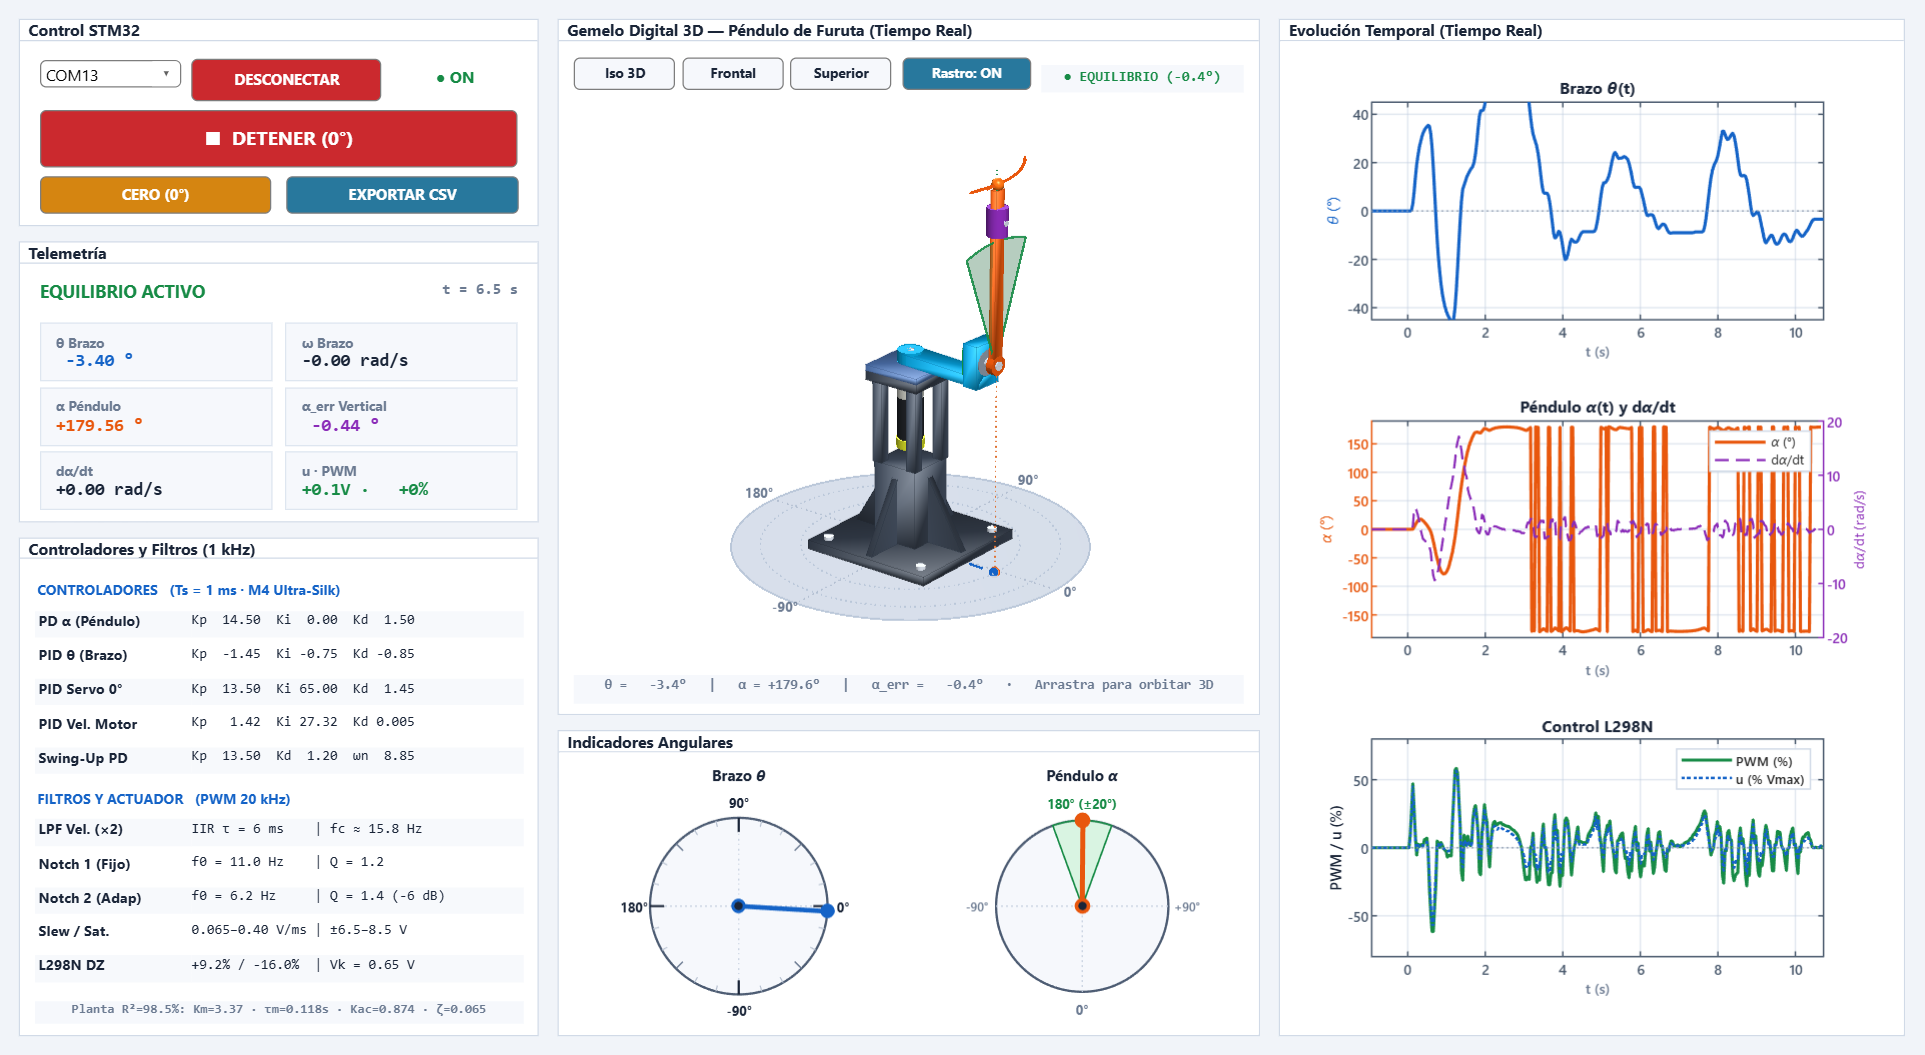
\includegraphics[width=0.78\textwidth]{fig_interfaz_matlab_gui.png}
    \caption{Interfaz gráfica MATLAB (\texttt{app\_telemetria\_sistema\_furuta\_matlab.m}): control único, KPIs y constantes (Col.~1), gemelo digital 3D \texttt{hgtransform} con rastro y diales polares (Col.~2) y series temporales en tiempo real (Col.~3).}
    \label{fig:interfaz_matlab}
\end{figure*}
